%%%%%%%%%%%%%%%%%%%%%%%%%%%%%%%%%%%%%%%%%%%%%%%%%%%%%%%%%%%%%%%%%%%%%%%%%%%%%%%%
% Universität Düsseldorf                                                       %
% Lehrstuhl für Softwaretechnik und Programmiersprachen                        %
% Vorlage für Bachelor- und Masterarbeiten                                     %
% Erstellt: 2019-09-03                                                         %
%%%%%%%%%%%%%%%%%%%%%%%%%%%%%%%%%%%%%%%%%%%%%%%%%%%%%%%%%%%%%%%%%%%%%%%%%%%%%%%%
\documentclass{hhuthesis}


%%%%%%%%%%%%%%%%%%%%%%%%%%%%%%%%%%%%%%%%%%%%%%%%%%%%%%%%%%%%%%%%%%%%%%%%%%%%%%%%
%% Einstellungen zur Personalisierung                                         %%
%%                                                                            %%
%% Im Folgenden können Sie Ihre Arbeit personalisieren.                       %%
%%%%%%%%%%%%%%%%%%%%%%%%%%%%%%%%%%%%%%%%%%%%%%%%%%%%%%%%%%%%%%%%%%%%%%%%%%%%%%%%

%% Spracheinstellung
%% Kommentieren Sie die entsprechende Zeile ein bzw. aus.
%% Wir empfehlen jedem sich an einer englischen Arbeit zu versuchen.
% \usepackage[ngerman,english]{babel} % English
\usepackage[english,ngerman]{babel} % Deutsch

%% Ihr Name
\author{Heiko Kauschke}

%% Der Titel der Arbeit
\title{The CART of Prolog: Implementierung von Entscheidungsbäumen mittels logischer Programmierung}
% \subtitle{Usually not needed}

%% Der zu erreichende Abschluss, entweder Bachelor oder Master
\graduationtype{Bachelor}
% \graduationtype{Master}

%% Ihr Studienfach
\subject{Informatik}

%% Beginn- und Abgabedaten der Arbeit
\begindate{02.~Juni~2022} % Beginn
\duedate{02.~September~2022} % Abgabe

%% Erst- und Zweitgutachter
\firstexaminer{Prof.~Dr.~Michael~Leuschel}
\secondexaminer{Prof.~Dr.~Stefan~Conrad}

%% Farb- oder Schwarzweißdruck
% Benutzen Sie das Kommando \blackwhiteprint,
% wenn sie in schwarzweiß drucken möchten.
% Im Farbdruck ist jede farbige Seite idR teurer.
% \blackwhiteprint % Kommentarzeichen entfernen für Schwarzweißdruck

%%%%%%%%%%%%%%%%%%%%%%%%%%%%%%%%%%%%%%%%%%%%%%%%%%%%%%%%%%%%%%%%%%%%%%%%%%%%%%%%
%% (Ende) Einstellungen zur Personalisierung                                  %%
%%%%%%%%%%%%%%%%%%%%%%%%%%%%%%%%%%%%%%%%%%%%%%%%%%%%%%%%%%%%%%%%%%%%%%%%%%%%%%%%
%% LaTeX Packages in Nutzung                                                  %%
%%                                                                            %%
%% Im folgenden können Sie für die Niederschrift Ihrer Arbeit benötigte       %%
%% LaTeX-Pakete einbinden.                                                    %%
%% Diese Vorlage kommt bereits mit einigen nützlichen inkludierten Paketen.   %%
%%%%%%%%%%%%%%%%%%%%%%%%%%%%%%%%%%%%%%%%%%%%%%%%%%%%%%%%%%%%%%%%%%%%%%%%%%%%%%%%

%% Macht den \todo-Befehl verfügbar.
%% Hiermit können Sie Abschnitte annotieren,
%% welche weiterer Bearbeitung bedürfen.
\usepackage[textsize=scriptsize]{todonotes}

%% Zeige Zeilennummern in der Arbeit an.
%% Der \linenumbers Befehl muss hierzu aufgerufen werden.
%% Praktisch für Feedback Ihrer potentiellen Korrekturleser!
\usepackage{lineno}
% \linenumbers % <- Kommentar entfernen!


%% Häufig benutzte mathematische Packages.
\usepackage{amsfonts}
\usepackage{amsmath}
\usepackage{amssymb}

\usepackage{siunitx} % \num Befehl zum einfacheren Formatieren von Zahlen.
\usepackage{enumitem} % Leichter konfigurierbare enumerate-Umgebungen.
\usepackage{subcaption} % Unterteilung von Figures in Subfigures.
\usepackage[colorlinks]{hyperref} % Klickbare Links (z.B. Inhaltsverzeichnis).
\sethyperrefpdfinfos{} % Setzt Autor, Titel, etc. als PDF-Metadaten.
\sethyperrefhhucolors{} % Setzt den Farbsatz der HHU für hyperref.
\usepackage{hypcap} % Ankert hyperref links auf Grafik/Tabelle statt Caption.
\usepackage{url} % \url Kommando für Darstellung von Links
\usepackage{csquotes} % Improved quoting.
\usepackage{microtype} % Verbessertes Kerning zwischen Wörtern.

%% Tabellen
\usepackage{tabularx} % tabularx Umgebung für mehr Kontrolle über Tabellen.
\usepackage{booktabs} % \toprule, \midrule, \bottomrule
\usepackage{multirow}
\usepackage{multicol}
\usepackage{longtable} % Große Tabellen gehen über mehrere Seiten.

%% Quellcode
\usepackage{listings} % Einbindung von Code.
\setlstlistingstyle{} % Kosmetische Einstellungen

%% Algorithmen in Pseudocode
\usepackage{algorithm} % Float-Umgebung für angegebene Algorithmen.
\usepackage{algorithmicx} % Angabe von Algorithmen in Pseudocode.
\usepackage{algpseudocode} % Standard Pseudocode-Elemente für Algorithmen.
\setalgorithmstyle{} % Kosmetische Einstellungen

%% Intelligenteres Referenzieren mittels \cref.
%% \languagename um dynamisch zwischen ngerman oder english zu wechseln.
\usepackage[\languagename,capitalize,noabbrev]{cleveref}

%%%%%%%%%%%%%%%%%%%%%%%%%%%%%%%%%%%%%%%%%%%%%%%%%%%%%%%%%%%%%%%%%%%%%%%%%%%%%%%%
%% (Ende) LaTeX Packages in Nutzung                                           %%
%%%%%%%%%%%%%%%%%%%%%%%%%%%%%%%%%%%%%%%%%%%%%%%%%%%%%%%%%%%%%%%%%%%%%%%%%%%%%%%%


\begin{document}
%% Set up title page, declaration of authorship, abstract, acknowledgements
\frontmatter
\makefrontmatter

%%%%%%%%%%%%%%%%%%%%%%%%%%%%%%%%%%%%%%%%%%%%%%%%%%%%%%%%%%%%%%%%%%%%%%%%%%%%%%%%
%% Danksagungen                                                               %%
%%%%%%%%%%%%%%%%%%%%%%%%%%%%%%%%%%%%%%%%%%%%%%%%%%%%%%%%%%%%%%%%%%%%%%%%%%%%%%%%
\begin{acknowledgements}
  Ich möchte mich herzlichst bei Jannik Dunkelau für die gute Betreuung bedanken.
  Zusätzlich danke ich allen, die meine Arbeit Probe gelesen haben und mir geholfen
  haben sie stets ein Stück besser zu machen.
\end{acknowledgements}
%%%%%%%%%%%%%%%%%%%%%%%%%%%%%%%%%%%%%%%%%%%%%%%%%%%%%%%%%%%%%%%%%%%%%%%%%%%%%%%%
%% (Ende) Danksagungen                                                        %%
%%%%%%%%%%%%%%%%%%%%%%%%%%%%%%%%%%%%%%%%%%%%%%%%%%%%%%%%%%%%%%%%%%%%%%%%%%%%%%%%


\tableofcontents


\mainmatter

%%%%%%%%%%%%%%%%%%%%%%%%%%%%%%%%%%%%%%%%%%%%%%%%%%%%%%%%%%%%%%%%%%%%%%%%%%%%%%%%
%% Der Inhalt der Arbeit                                                      %%
%%                                                                            %%
%% Hier können Sie die schriftliche Ausarbeitung ihrer Arbeit                 %%
%% niederschreiben. Der Übersicht halber bietet sich jedoch an, dies in einer %%
%% oder mehreren separaten Dateien zu tun, welche mittels \input eingebunden  %%
%% werden --- wie auch in der Vorlage geschieht.                              %%
%%%%%%%%%%%%%%%%%%%%%%%%%%%%%%%%%%%%%%%%%%%%%%%%%%%%%%%%%%%%%%%%%%%%%%%%%%%%%%%%

%%%%%%%%%%%%%%%%%%%%%%%%%%%%%%%%%%%%%%%%%%%%%%%%%%%%%%%%%%%%%%%%%%%%%%%%%%%%%%%%
% Diese Datei beinhaltet den eigentlichen Inhalt Ihrer Arbeit.
%
% Es bietet sich der Übersicht halber an, die einzelnen Abschnitte jeweils
% in eigene Dateien zu schreiben und mittels \input einzubinden.
% Eine mögliche Verzeichnisstruktur sähe entsprechend so aus:
%
%     thesis/
%     +- tex/
%     |  +- introduction.tex
%     |  +- motivation.tex
%     |  +- experiments.tex
%     |  |  ...
%     |  +- conclusion.tex
%     +- abstract.tex
%     +- contents.tex
%     +- thesis.tex
%%%%%%%%%%%%%%%%%%%%%%%%%%%%%%%%%%%%%%%%%%%%%%%%%%%%%%%%%%%%%%%%%%%%%%%%%%%%%%%%

\section{Einleitung}

Das Schlagwort maschinelles Lernen hat durch die heutzutage zur Verfügung stehende Rechenleistung,
immer mehr Aufmerksamkeit gefunden. Zudem ist durch das Internet die Sammlung von Daten sehr viel leichter
geworden und es stehen ausreichend Daten zur Verfügung, die analysiert werden können.
Um diese Daten zu verarbeiten werden gerne Klassifikationsalgorithmen benutzt. Diese finden nicht nur
Verwendung im Bereich des Data-Mining~\cite{sharma2016survey}, sondern auch in klinischen Studien~\cite{lewis2000introduction}
und der psychologischen Forschung~\cite{Strobl2009-hw}.
In diesen Feldern wird für die Klassifikation ein sogenannter Entscheidungsbaum benutzt.
Entscheidungsbäume sind in den eben genannten Gebieten beliebt, da sie sich leicht grafisch darstellen lassen
und die Regeln, nach denen klassifiziert wird, ablesbar und leicht verständlich sind.
Die zwei bekanntesten Algorithmen zur Erstellung von Entscheidungsbäumen sind schon lange im Umlauf.
Der CART-Algorithmus~\cite{breiman1984classification} wurde von Breiman im Jahr 1984 und C4.5, von Quinlan, im Jahr 1993~\cite{quinlan1993c45}
vorgestellt. CART lässt sich sogar für sogenannte Regressionsprobleme verwenden, wodurch für eine Eingabe auch ein stetiger Wert
vorhergesagt werden kann anstatt einer Klasse. Dieser Algorithmus ist folglich auch in verschiedenen Bibliotheken für maschinelles Lernen,
in verschiedenen Programmiersprachen, implementiert. Allerdings nicht in Prolog.

Prolog~\cite{Colmerauer1993TheBO} ist eine logische Programmiersprache und spielt eine große Rolle beim Bau von Expertensystemen~\cite{merritt2012building}
und wird heutzutage gerne im Bereich der künstlichen Intelligenz~\cite{shoham2014artificial} und diversen anderen Feldern~\cite{806816,wicaksono2016relational} eingesetzt.
Diese Programmiersprache besitzt keine Standard Bibliothek für Algorithmen des maschinellen Lernens, trotz seiner wichtigen Rolle in der künstlichen Intelligenz.
Da der CART-Algorithmus rekursiv ist, macht es durchaus Sinn diesen Algorithmus, in Prolog umzusetzen, da diese Programmierspache
hervorragend mit Rekursion umgehen kann. Zusätzlich würde eine Implementierung eines Entscheidungsbaums in Prolog zeigen, ob es sinnvoll ist
Machine-Learning-Algorithmen in puren Prolog zu implementieren.

In dieser Arbeit soll untersucht werden, wie gut eine pure Prolog Implementierung des Entscheidungsbaum Algorithmus
CART, im Vergleich zu den weit verbreiteten Referenzimplementierungen aus Python und R ist.
Dafür wird zunächst das benötigte Wissen über die benutzten Algorithmen und Prolog eingeführt.
Daraufhin wird die Implementierung und anschließend die Ergebnisse eines Performancevergleichs vorgestellt.

\section{Grundlagen}
In diesem Kapitel werden die benötigten Konzepte und Algorithmen erklärt, die für das Verständnis der Arbeit notwendig sind.
In \cref{sec:entscheidungsbaum} wird auf die grundlegende Funktionsweise von Entscheidungsbaum-Algorithmen, in speziellem den CART-Algorithmus, eingegangen.
Daraufhin wird in \cref{sec:randomforest} das Vorgehen von Random-Forest-Algorithmen beschrieben. In \cref{sec:prolog}
wird die Programmiersprache Prolog kurz eingeführt.


\subsection{Entscheidungsbaum} \label{sec:entscheidungsbaum}
Entscheidungsbaumalgorithmen sind sogenannte nicht-parametrische Methoden, das heißt, dass vor der
Entstehung des Baums keine Parameter vorgegeben werden müssen und die Struktur des Baums von den Daten abhängt.
Ein Entscheidungsbaum ist eine hierarchische Struktur die aus internen Entscheidungsknoten und terminalen Blättern besteht.
Jeder Entscheidungsknoten beinhaltet eine einfache Funktion mit diskreten Ergebnissen, die die Zweige repräsentieren.
Diese Funktionen werden so gewählt, dass sie den Eingaberaum in immer kleinere Regionen unterteilen, welche wiederum
unterteilt werden, je weiter man den Pfad von der Wurzel nach unten folgt.
Ein terminales Blatt entsteht dann, wenn die lokale Region im Eingaberaum nicht weiter unterteilt werden soll.
Im Falle von Klassifikationsbäumen ist das meist der Fall, wenn die Region nur aus den gleichen diskreten Werten besteht,
während es bei Regressionsbäumen sehr ähnliche stetige Werte sind.
Ein beispielhafter Entscheidungsbaum und die dazugehörige Unterteilung des Eingaberaums ist in \cref{fig:baum}~\cite{Alpaydin+2022} dargestellt.
\begin{figure}[h]
  \centering
  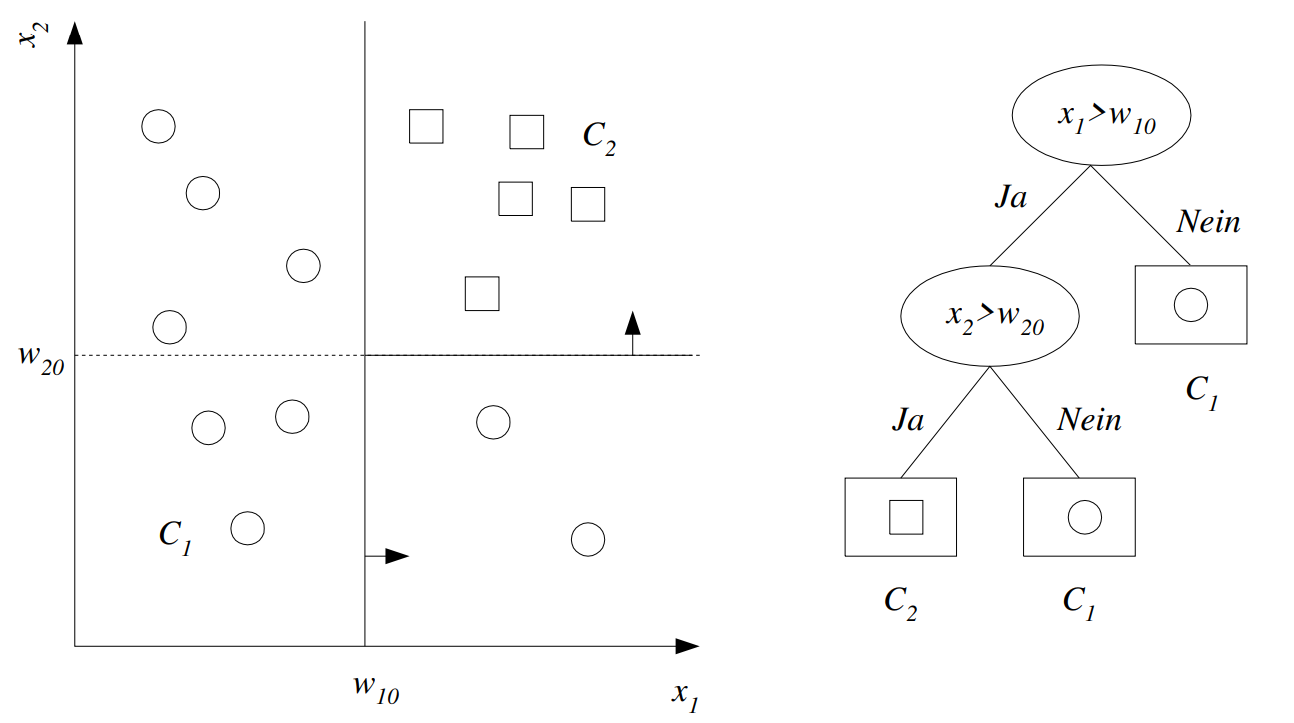
\includegraphics[width=10cm]{fig/baum.png}
  \caption{beispielhafter Entscheidungsbaum und Unterteilung. Ovale sind Entscheidungsknoten, Vierecke sind Blattknoten.}%
  \label{fig:baum}
\end{figure}
Bei gegebener Eingabe wird nun an jedem Knoten das Ergebnis der entsprechenden Funktion berechnet. In Abhängigkeit von dem Ergbnis
wird daraufhin der Zweig ausgewählt, welcher entlang gegangen wird. Das wird so lange wiederhohlt, bis man an in einem
Blattknoten angekommen ist. Der in diesem Blatt stehende Wert wird dann als Ausgabe benutzt.

In dieser Arbeit geht es um den CART Algorithmus, deswegen wird im Folgenden
nur die typische Vorgehensweise~\cite{CRAWFORD1989197} für diesen Algorithmus vorgestellt.
Diese ist in \cref{alg:baum} exemplarisch dargestellt.
\begin{algorithm}
  \caption{Training eines Entscheidungsbaums}%
  \label{alg:baum}
  \begin{algorithmic}[1]
    \Function{CreateTree}{Data}
      \If{\Call{Abbruchbedingung}{D} \(=\) true}
        \State label \(\gets\) \Call{Klasse}{D}
        \State \Return label
      \EndIf
      \State bestValue \(\gets \infty\)
      \State \(\mathit{bestSplit} \gets \) NIL
      \State splits \(\gets\) \Call{erstelleSplitliste}{D}
      \ForAll{\(s \in splits\)}
        \State \(\mathit{value} \gets \) \Call{KombiniertGini}{D, s}
        \If{\(\mathit{value} < \mathit{bestValue}\)}
          \Comment{Aktualisiere besten Wert}
          \State \(\mathit{bestValue} \gets \mathit{value}\)
          \State \(\mathit{bestSplit} \gets s\)
        \EndIf
      \EndFor
      \State leftTree, rightTree \(\gets\) \Call{aufteilen}{D,bestSplit}
      \State leftRes \(\gets\) \Call{CreateTree}{leftTree}
      \State rightRes \(\gets\) \Call{CreateTree}{rightTree}
      \State \Return \((s, leftRes, rightRes)\)
    \EndFunction
  \end{algorithmic}
\end{algorithm}
Der Baum besteht ursprünglich nur aus einen Wurzelknoten und beinhaltet den gesamten Datensatz T.
Als erstes wird die Menge aller möglichen binären Aufteilungen, von T, durchsucht, bis eine optimale
gefunden wurde. Was eine optimale Aufteilung ist, wird dabei durch ein Maß der Unreinheit bestimmt, welches minimiert
werden muss. Typischerweise benutzt der CART Algorithmus den Gini-Index für Klassifikation, abgebildet in \cref{eq:gini}.
Im Falle der Regression wird meist die Residuenquadratsumme benutzt, abgebildet in \cref{eq:rss}.
\begin{align}
    Gini(T)       & = 1 - \sum_{i=1}^n p_i^2 \label{eq:gini} \\
    \mathit{RSS}(T)       & = \sum_{i=1}^n (\bar{y} - x_i)^2 \label{eq:rss} 
  \end{align}
Hier ist \(p_i\) die relative Häufigkeit von der i-ten Klasse in T, während \(\bar{y}\) das arithmetische Mittel der Zielvariablen
in T ist und \(x_i\) die Zielvariable des i-ten Datenpunkts in T.
Diese Maße werden benutzt um die Reinheit eines einzelnen Knoten zu messen.
Um eine optimale Aufteilung zu finden, zum Beispiel, im Fall der Klassifikation mit Gini-Unreinheit,
muss \cref{eq:combgini} minimiert werden.
\begin{align}
    Gini(T)_{Split}       & = N_1/N * Gini(T_1) + N_2/N * Gini(T_2) \label{eq:combgini}
  \end{align}
Hier ist der Datensatz T in zwei Teile, \(T_1\) und \(T_2\), aufgeteilt und \(N_1\) und \(N_2\) geben die Anzahl an Datenpunkten
in der jeweiligen Teilmenge an.
Eine Aufteilung durch stetige Attribute nimmt dabei eine Regel der Form,
 \(A \leq r\) 
an, wobei r die Mitte von zwei beliebigen, unterschiedlichen Datenpunkten ist. Für ein kategorisches Attribut, welches die Werte
\(D_1\) bis \(D_n\) annehmen kann, nimmt die Aufteilung die Form \(A \in D_T\) an, wobei \(D_T\) eine Teilmenge von \{\(D_1\),...,\(D_n\)\} ist.
Nachdem eine optimale Aufteilung gefunden wurde, werden zwei Nachfolgerknoten, für den Wurzelknoten, erstellt.
Der linke enthält die Datenpunkte aus dem Datensatz, die die Regeln erfüllen, während der rechte den restlichen
Datensatz enthält.
Dieser Prozess nun wird rekursiv auf jedes Blatt angewendet, bis eine Abbruchbedingung erreicht ist. Eine Abbruchbedingung
kann einsetzen, wenn der Datensatz in einem Blatt zu klein ist, nur noch eine Klasse in allen Datenpunkten vertreten ist oder
sich die Datenpunkte nicht mehr unterscheiden lassen.
Da ein Entscheidungsbaum in den meisten Fällen unter \enquote{overfitting} leidet, wird dieser am Ende gestutzt.
Das Pruning ist ein komplexer Vorgang, der nicht in meiner Implementierung angewandt wurde, deswegen wird hier nicht näher
darauf eingegangen.

\subsection{Random Forest} \label{sec:randomforest}
Nach Breiman ist ein Random Forest \cite{Breiman2001} ein Klassifikator der aus einer Sammlung von
baumartigen Klassifikatoren besteht, welche aus unabhängig identisch verteilten Zufallsvektoren erstellt wurden,
und jeder Baum stimmt für die beliebteste Klasse der Eingabe.
Random Forest gehört zu den sogenannten \enquote{Ensemble Methoden}. Der Gedanke hinter diesen Methoden ist es,
das Problem der Instabilität von Entscheidungsbäumen zu lösen~\cite{Strobl2009-hw}, indem, bei Vorhersagen, der Durchschnitt von mehreren Bäumen genommen
wird. Durch diese Technik soll auch das Problem gelöst werden, dass Entscheidungsbäume sehr empfindlich gegenüber Änderungen
im Trainingsdatensatz reagieren.

Ein Random-Forest-Algorithmus besteht aus zwei Hauptbestandteilen: Bagging~\cite{breiman1996bagging} und
Feature Randomness.
Bagging (\enquote{bootstrap aggregating}) ist ein Verfahren das 1996 von Breiman vorgestellt wurde um
die Präzision von instabilen Verfahren, wie Entscheidungsbäumen, zu verbessern.
Beim bagging werden aus einem N großen Datensatz, N zufällige Instanzen mit zurücklegen gezogen.
Diese N Instanzen werden dann als Datensatz benutzt um einen Klassifikator zu trainieren. Dieser Vorgang
wird mehrfach wiederholt, bis man genug Klassifikatoren trainiert hat.
Um eine Vorhersage zu treffen, wird eine Vorhersage von allen Klassifikatoren getroffen. Anschließend
wird für die finale Vorhersage ein Mehrheitsentscheid getroffen, wobei alle Klassifikatoren eine Stimme haben.
Bei einem Random Forest sind diese Klassifikatioren Entscheidungsbäume.

Jedoch werden die Klassifikatoren nicht nur mit einem zufällig erzeugten Datensatz trainiert.
Bei dem Training von Entscheidungsbäumen in einem Random Forest wird zudem Feature Randomness eingesetzt.
Das heißt, dass bei der Konstruktion nicht alle Attribute der Instanzen im Datensatz genutzt werden.
Stattdessen wird voher eine zufällige Teilmenge aller Attribute erstellt, die während des Trainings benutzt werden.
Wie groß die Teilmenge ist, hängt davon ab, ob ein Klassifikationsbaum oder Regressionsbaum trainiert wird.
In \enquote{The Elements of Statistical Learning: Data Mining, Inference, and Prediction} wird vorgeschlagen,
dass man im Falle der Klassifikation \cref{eq:att-klass} und der Regression \cref{eq:att-reg} benutzt.
Hier ist m die Anzahl der Attribute, die eine Instanz besitzt.
\begin{align}
    M_{Klassifikation}       & = \lfloor\sqrt{m}\rfloor \label{eq:att-klass} \\
    M_{Regression}       & = \lfloor{m/3}\rfloor \label{eq:att-reg}
  \end{align}
Somit wird in einem Random-Forest-Algorithmus in jedem Schritt ein Entscheidungsbaum, mithilfe eines zufällig
erstellten Datensatz, der auf einem Eingabe Datensatz basiert, und einer zufälligen Teilmenge von Attributen erstellt,
bis die gewünschte Anzahl an Entscheidungsbäumen erreicht ist.
Um eine Vorhersage mit einem Random Forest zu treffen, wird eine Vorhersage von jedem Baum getroffen.
Im Falle der Klassifikation wird die Vorhersage nach einem Mehrheitsentscheid getroffen und im Falle der Regression
wird das arithmetische Mittel aller Vorhersagen ermittelt.

\subsection{Prolog} \label{sec:prolog}
Prolog~\cite{Colmerauer1993TheBO} ist eine Programmiersprache, die 1972 von dem französichen Informatiker Alain Colmerauer maßgeblich entwickelt wurde.
Sie ermöglicht deklaratives Programmieren und gilt als die wichtigste logische Programmierspache.
Das Einsatzfeld befindet sich, auch historisch, in den Expertensystemen~\cite{merritt2012building}, aber auch
beim Theorem Proving~\cite{zombori2020prolog} und Model Checking~\cite{sridhar2010actionscript}, um ein paar
Beispiele zu nennen.

Als logische Programmiersprache ist Prolog deklarativ und nicht imperativ, wie zum Beispiel die Pogrammiersprachen Java und C.
In Prolog Programmen wird beschrieben was berechent wird und nicht wie.
Die Grundlagen eines Prolog Programms sind Fakten und Regeln.
Fakten sind Aussagen, die ohne Bedingung wahr sind und bestehen nur aus einem Kopf. Regeln bestehen aus einem Kopf und einem Rumpf.
Im Rumpf können endlich viele Aussagen stehen, die logisch verknüpft sind.
Die logischen Verknüpfungen in Prolog sind in \cref{table:logic} abgebildet.
\begin{table}[ht]
  \begin{center}
    \caption{logische Verknüpfungen in Prolog}
    \label{table:logic}
    \begin{tabular}{cc}
      \toprule
      Verknüpfung   & Prolog \\
      \midrule
      \(\Leftarrow\)      &  :-    \\
      \(\wedge\)         &  ,    \\
      \(\vee\)         &  ;    \\
      \(\neg\)         &  \textbackslash+    \\
      \bottomrule
    \end{tabular}
  \end{center}
\end{table}
Relevant für meine Implementierung sind Prädikate. Ein Prädikat p hat die Arität n, wobei n die Anzahl der Datenwerte ist,
die das Prädikat bekommt. Ein Prädikat, das als Fakt geschrieben ist, also nur als Kopf, ist immer wahr.
Wenn es als Regel geschrieben ist, ist das Prädikat nur wahr, wenn der Rumpf wahr ist.
Zudem dürfen logische Verknüpfungen, wie \(\wedge\), \(\vee\) und \(\neg\) nur im Rumpf verwendet werden.
Das sorgt dafür, dass, wenn man die Implikation zwischen Kopf und Rumpf auflöst, der Kopf das einzige positive Literal darstellt und
die restlichen Terme, negative Literale.
Die Datenwerte, die in ein Prädikat hinein gegeben werden können, können im Programmcode aus Variablen bestehen.
Variablen fangen mit Großbuchstaben oder einem Unterstrich an. Wichtig zu beachten ist, dass der Datenwert einer Variable
nicht verändert werden kann, sollte es jedoch zu Backtracking kommen, kann es sein, dass die Variable in einem anderen Teilbaum,
mit einem anderen Datenwert unifiziert wird.
Rekursion von Prädikaten ist erlaubt und wird bei der Ausführung von Programmcode unter gewissen Umständen von Prolog performance technisch
optimiert.
Für meine Implementierung werden außerdem Komplexe Werte, oder auch compound Terms genannt, gebraucht.
Diese bestehen aus einem Funktor f mit einer Stelligkeit von n.
Im Gegensatz zu Prädikaten stehen sie für neue Datenwerte und stellen einen Term dar.
Ob f(a,b) ein Prädikat oder ein Term ist, hängt letzendlich von der Position in der Klausel ab.

Prolog besitzt die Eigenschaft der Homoikonizität. Somit sind Programme gleichzeitig auch Datenstrukturen. 
Jedoch bietet Prolog, durch eine spezielle Schreibweise, gewisse Vorteile für die Benutzung einer Liste als Datenstruktur.
Eine Liste wird durch [] umschlossen und
kann beliebig viele Elemente beinhalten, welche alle von unterschiedlichen Typen sein können.
Bei der Verarbeitung von Listen, wird meist die eingebaute Head-Tail-Aufteilung benutzt. Dabei wird das erste Element der Liste
mit der Head-Variable unifiziert, während die restliche Liste mit der Tail-Variable unifiziert wird.
\cref{lst:list} zeigt das in SWI-Prolog~\cite{wielemaker:2011:tplp} eingebaute Prädikat \texttt{is\_list/1} und
demonstriert ein einfaches Prolog Programm, dass überprüfen soll, ob die Eingabe eine Liste ist oder nicht.
\begin{lstlisting}[
  float, caption={Prolog implementation of \texttt{is\_list/1}},
  label={lst:list}, language=Prolog
]
is_list(X) :-
        var(X), !,
        fail.
is_list([]).
is_list([_|T]) :-
        is_list(T).
\end{lstlisting}
Das Prädikat \texttt{is\_list/1} wird hier zweimal als Regel und einmal als Fakt verwendet.
Bei einem Programmaufruf wird zuerst die oberste Regel aufgerufen. Diese unifiziert die Eingabe mit der Variable
X. Das sorgt dafür, dass diese Eingabe auch von \texttt{var/1} benutzt wird. Diese Prädikat wird wahr, wenn die Eingabe
eine Variable ist und schlägt sonst fehl.
Sollte das Programm an der Stelle fehlschlagen, wird als nächstes der Fakt überprüft, da Regeln Hornklauseln
darstellen und bei etwas im Rumpf falsch ist, die Regel falsch ist.
Falls die Eingabe tatsächlich eine Variable ist, ist \texttt{var/1} wahr und der sogenannte Cut (!) wird eingelesen.
Dieser verhindert, dass Backtracking betrieben wird. In dem Fall würde durch das fail die Regel falsch sein und durch den Cut
wird der Fakt und die andere Regel nicht mehr überprüft und das Programm gibt falsch aus.
Falls die leere Liste die Eingabe ist, gibt das Programm in dem Moment wahr aus, wenn es den Fakt liest.
Wenn das Programm mit einer Liste, die nicht leer ist, aufgerufen wird, wird auch die letzte Regel erreicht.
Diese kann nur aufgerufen werden, wenn sich die Eingabe in die Head-Tail-Aufteilung zerlegen lässt.
Hier wird der Kopf mit einer sogenannten anonymen Variable unifiziert und der Tail mit der Variable T.
Als nächstes wird dann überprüft ob T eine Liste ist. Diese Überprüfung wird somit rekrusiv so lange ausgeführt,
das Prädikat fehlschlägt oder der Fakt erreicht wird. 

\section{Implementierung}
In diesem Kapitel wird zunächst der selbst angefertigte Quellcode
für den CART Algorithmus ausführlich erklärt. Darufhin folgt der Code für den
Random Forest Algorithmus. Zum Schluss wird noch auf den Code eingegangen, der benötigt wird um
Vorhersagen mit den erzeugten Strukturen zu Treffen.

\subsection{Entscheidungsbäume}
Vorab muss erwähnt werden, dass die Art wie ich meinen Baum und den Datensatz repräsentiere,
auf der Code-Skizze zu Entscheidungsbäumen
aus dem Buch \enquote{Prolog programming for artificial intelligence}~\cite{bratko2001prolog}, basiert.
Wie das aussieht ist in \cref{table:Struktur} dargestellt.
\begin{table}[ht]
  \begin{center}
    \caption{Darstellung von Baum und Datensatz}
    \label{table:Struktur}
    \begin{tabular}{cc}
      \toprule
      Strukur   & Darstellung \\
      \midrule
      Baum      &  \(tree(Attribut = Wert, LinkerTeilbaum, RechterTeilbaum)\)    \\
      Datensatz   &  \([example(Klasse, [Att1 = Wert1,...]), example(...), ...]\)  \\
      \bottomrule
    \end{tabular}
  \end{center}
\end{table}

Analog zu der Erklärung zum Algorithmus, wird die Implementierung von oben nach unten erklärt.
Im ersten Prädikat, \cref{lst:induce-tree}, befindet sich der rekursive Aufruf der den Baum konstruiert.
Der erste Fall gibt einen leeren Baum, beziehungsweise Liste, zurück, falls keine Daten übergeben wurden.
Der zweite Fall überprüft, ob alle momentan genutzten Datenpunkte dieselbe Klasse haben, wie der erste Datenpunkt
in der Liste. Dafür wird das Hilfsprädikat \texttt{check-classes/2} verwendet. Falls dies der Fall sein sollte wird ein Blatt erzeugt.
Der dritte Fall erzeugt zwei Kinder im Entscheidungsbaum. Dafür wird zuerst, mithilfe von \cref{lst:find-best-split},
aus den vorhandenen Datenpunkten, ein Wert zu einem Attribut gefunden, der am besten zwischen den Klassen
differenziert. Daraufhin wird mit Hilfe dieses Attribut-Wert-Paares und \texttt{split/4} der Datensatz entsprechend aufgeteilt.
Der Wert von dem gefundenen Attribut-Wert-Paar ist im numerischen Fall eine Zahl und im kategorischen Fall eine Teilmenge der Werte,
die das entsprechende Attribut annehmen kann.
Dabei landen die Datenpunkte, bei numerischen Werten, die kleiner sind als der gegebene Wert, im linken ansonsten im rechten Teilbaum.
Bei kategorischen Werten landen die Datenpunkte im linken Teilbaum, wenn deren Werte, teil der Teilmenge sind, ansonten im rechten.
Die daraus entstehenden Teilmengen werden dann genutzt um Teilbäume zu konstruieren.
Im Gegensatz zu den üblichen Implementierungen habe ich mich dazu entschieden den Baum bis zur höchsten Reinheit aufzubauen.
Zum einen besteht laut Demidova und Usachev~\cite{Demidova_2020} die Gefahr, dass bei anderen Abbruchbedingungen
die Klassifikations-Qualität verloren geht und zum anderen muss kein extra Quellcode für die Verwendung von Random Forest
angefertigt werden.
Jedoch gibt es eine weitere Abbruchbedingung die eingebaut werden musste. Falls der aktuelle Datensatz Datenpunkte
enthält, die von verschiedenen Klassen sind, sich aber nicht unterscheiden lassen, wird ein Blatt erzeugt.
Bei Klassifikationsbäumen hat das Blatt die Klasse, die am meisten im Datensatz vertreten ist, bei Regressionsbäumen
ist das Blatt das arithmetische Mittel der Zielvariablen im Datensatz.
\begin{lstlisting}[
    float, caption={Prolog implementation of \texttt{induce\_tree/3}},
    label={lst:induce-tree}, language=Prolog
  ]
%! induce_tree(+Daten:list, +Attribute:list, -Tree:term) is det
%
%  induziert den Entscheidungsbaum durch 3 verschiedene Faelle:
%  1) Tree = null, wenn keine Daten existieren
%  2) Tree = leaf(Class), wenn alle Beispiele zur selben Klasse gehoeren
%            oder nicht mehr unterschieden werden koennen
%  3) Tree = tree(Attribut = Wert, SubTree1, SubTree2), wenn es mehr als
%            eine vorhandene Klasse gibt.
induce_tree([], _, []) :- !.
induce_tree([example(Klasse, _)|T], _, leaf(Klasse)) :-
    check_classes(T, Klasse), !.
induce_tree(Daten, Attribute, tree(BestAttVal, SubTree1, SubTree2)) :-
    find_best_split(Daten, Attribute, BestAttVal),
    split(Daten, BestAttVal, Split1, Split2),
    induce_tree(Split1, Attribute, SubTree1),
    induce_tree(Split2, Attribute, SubTree2).
induce_tree(Daten, Attribute, leaf(Klasse)) :-
    find_best_split(Daten, Attribute, err = Klasse), !.
\end{lstlisting}

Als nächstes geht es darum das beste Attribut-Wert-Paar zum aufteilen des Datensatzes zu finden.
Dieser Schritt lässt sich in zwei Teilschritte unterteilen. Als erstes muss eine Liste erstellt werden,
die die Attribut-Wert Paare beinhaltet an denen der Datensatz potentiell aufgeteilt werden kann.
Als zweites muss das Paar ausgewählt werden, welches die zwei \enquote{reinsten} Datensätze hervorbringt.
Die Koordinierung dieser beiden Aufgaben wird von \cref{lst:find-best-split} übernommen.
In der Implementierung wird an dieser Stelle die eben erwähnte Abbruchbedingung abgefangen.
Sollte \texttt{split\_candidates/2} eine leere Kandidatenliste ausgeben, ist klar, dass der aktuelle
Datensatz nicht weiter aufgeteilt werden kann. In dem Fall wird wie beschrieben vorgegangen.
\begin{lstlisting}[
    float, caption={Prolog implementation of \texttt{find\_best\_split/3}},
    label={lst:find-best-split}, language=Prolog
  ]
%! find_best_split(+Daten:list, +Attribute:list, -BestAttVal:Att = Val)
%  is det
%
% Findet den besten Split zur aktuellen Datenlage
find_best_split(Daten, Attribute, BestAttVal) :-
    split_candidates(Daten, Attribute, Kandidaten),
    ([] \= Kandidaten ->
        best_split(Kandidaten, Daten, BestAttVal)
    ;   get_classes(Daten, Klassen),
        sort(Klassen, Klassenliste),
        get_max(Klassenliste, Klassen, Max),
        best_split(Max, err, BestAttVal)).
\end{lstlisting}

Das erstellen der Liste von potentiellen Aufteilungen wird von \texttt{split\_candidates/3} erledigt.
Dieses Prädikat benutzt einen Akkumulator. Das heißt, dass es ein Prädikat mit seinen
Variablen und einer zusätzlichen leeren Liste aufruft. Hier wird mithilfe von \cref{lst:split-candidates-attribute}
eine Liste von Kandidaten für ein einzelnes Attribut erstellt. Diese Liste wird
an den Akkumulator angehangen. Das wird so lange wiederholt, bis alle Attribute abgearbeitet sind.
Dann wird der Akkumulator mit der Ausgabevariablen unifiziert.

Um eine Liste der Kandidaten zu erstellen, geht \cref{lst:split-candidates-attribute} wie folgt vor:
Zunächst wird durch \texttt{check\_attribute\_number/2} überprüft, ob das Attribut numerisch oder kategorisch ist.
Bei numerischen Werten wird \texttt{get\_values\_n/3} aufgerufen.
Hier wird wieder ein Akkumulator benutzt in dem die Werte zu dem aktuellen Attribut eingefügt werden.
Dabei wird darauf geachtet, dass kein Wert, zu einem Attribut, doppelt vorkommt.
Bei kategorischen Werten wird \texttt{get\_values\_k/3} aufgerufen. Hier wird analog
zum vorherigen Prädikat vorgegangen.
Nachdem eine Liste mit unterschiedlichen Werten vorliegt, berechnet \texttt{create\_candidates/3} daraus eine Liste mit möglichen Aufteilungen.
Im numerischen Fall wird dabei die Mitte von zwei Werten aus der übergebenen Liste berechnet und als
Attribut-Wert Paar in die Ergebnisliste aufgenommen. Im kategorischen Fall werden mit Hilfe von \texttt{my\_powerset/2}
mindestens \(2^{m-1} - 1\) verschiedene Kombinationen von Werten aus der Kandidaten Liste erzeugt, wobei m die Anzahl an Werten ist,
die das Attribut annehmen kann.
Dabei ist jede Kombination in einer Liste verpackt und wird dann als Attribut-Liste-Paar
in die Ergebnisliste aufgenommen.
Dadurch beinhaltet die Liste alle möglichen Kandidaten zur Aufteilungen des aktuellen Datensatzes.
Alternativ hätte man bei numerischen Werten das Minimum und Maximum nehmen können und in diesem Intervall
eine feste Anzahl an Aufteilungen, in gleichmäßigen Abständen durchführen können~\cite{breiman1984classification}.
Mola \cite{MOLA1997} hat auch schon einen schnelleren Aufteilungsalgorithmus vorgestellt, der auf dem Vorhersehbarkeits
Index basiert.

\begin{lstlisting}[
    float, caption={Prolog implementation of \texttt{split\_candidates\_attribute/3}},
    label={lst:split-candidates-attribute}, language=Prolog
  ]
%! split_candidates_attribute(+Daten:list, +Attribut:atom, -Kandidaten:list)
%  is det
%
%  Erstellt ein Liste mit allen moeglichen Splits zu einem Attribut
split_candidates_attribute(Daten, Attribut, Kandidaten) :-
    (check_attribute_number(Daten, Attribut) -> 
    get_values_n(Daten, Attribut, Values)
    ; get_values_k(Daten, Attribut, Values)),
    create_candidates(Values, Attribut, Kandidaten).
\end{lstlisting}

Mit der Liste aller möglichen Aufteilungen wird durch \cref{lst:best-split} die Aufteilung vom Datensatz gefunden,
die das Maß der Unreinheit minimiert. Im ersten Fall wird die Abbruchbedingung abgefangen und die Klasse für das Blatt nach oben gegeben.
Ansonsten werden die Unreinheit der Aufteilung, die durch den ersten
Kandidaten entsteht, und der Kandidat selbst, je als Variable gemerkt. Danach wird in jedem Schritt die Unreinheit
eines neuen Kandidaten berechnet und mit der entsprechenden Variable verglichen. Wenn der Wert kleiner ist,
wird mit diesem in den nächsten Schritten verglichen und der Kandidat wird auch gemerkt. Falls der neue Wert
der Unreinheit größer ist, werden die Variablen nicht überschrieben und es geht mit dem nächsten Kandidaten weiter.

\begin{lstlisting}[
  float, caption={Prolog implementation of \texttt{best\_split/3}},
  label={lst:best-split}, language=Prolog
]
%! best_split(+Kandidaten:list, +Daten:list, -BestAttVal: Att = Val)
%  is det
%! Kandidaten = [Att = Val1, Att = Val2, ...]
%
%  Verwendet alle Kandidaten aus der Liste um den besten Split
%  zu finden und auszugeben
best_split(Klasse, err, err = Klasse).
best_split([H|T], Daten, Res) :-
    impurity(Daten, H, Min),
    best_split(T, Daten, Min, H, Res).
best_split([], _, _, Res, Res) :- !.
best_split([H|T], Daten, Min, Cur, Res) :-
    impurity(Daten, H, CombUnreinheit),
    (CombUnreinheit < Min ->
        best_split(T, Daten, CombUnreinheit, H, Res)
    ;   best_split(T, Daten, Min, Cur, Res)).
\end{lstlisting}

Entscheidend ist auch, welches Maß der Unreinheit verwendet wird.
Dieses wird hinter dem Prädikat \cref{lst:impurity} versteckt.
\begin{lstlisting}[
  float, caption={Prolog implementation of \texttt{impurity/3}},
  label={lst:impurity}, language=Prolog
]
%! impurity(+Daten:list, +AttVal:Attribute = Value, -Unreinheit:double) is  det
%
%  Gibt die kombinierte Unreinheit, von dem Split des Datensatzes, aus
impurity(Daten, AttVal, CombUnreinheit) :-
    split_class(Daten, AttVal, Split1, Split2),
    combgini(Split1, Split2, CombUnreinheit).
\end{lstlisting}
In dieser Implementierung wird die \enquote{Gini-Unreinheit} verwendet.
Doch bevor gerechnet werden kann, bereitet \texttt{split-class/3} die Daten entsprechend auf.
Dieses Prädikat erstellt aus dem übergebenen Datensatz, mithilfe eines Attribut-Wert Paars, zwei kleinere Datensätze.
Die kleineren Datensätze bestehen dabei nur aus den Klassen der Datenpunkte, die in dem Datensatz zugeordnet wurden.
Dafür werden wieder 2 Akkumulatoren verwendet. Im ersten Fall wird zunächst nach dem Attribut vom Attribut-Wert-Paar
im Datensatz gesucht. Sobald dieses gefunden ist, gibt es einen Fall dafür, dass der Wert zu diesem
Attribut kategorisch oder numerisch ist. Im numerischen Fall wird überprüft, ob der Wert des Datenpunktes kleiner ist,
als der des übergebenen Werts. Falls dies der Fall ist, wird die Klasse des Datenpunktes an den linken Akkumulator angehangen,
ansonsten am rechten. Analog dazu wird mit kategorischen Werten umgegangen, nur das hier überprüft wird, ob
der Wert des Datenpunkts in der Liste der übergebenen Werte vorhanden ist.

Nach der Erstellung, der aus Klassen bestehenden Datensätze, berechnet \cref{lst:combgini}
die kombinierte Gini-Unreinheit der beiden Datensätze. Als erstes wird die Gini-Unreinheit der
einzelnen Datensätze mit \texttt{gini/2} berechnet. Die Ergebnisse daraus werden dann mit dem Anteil
an Datenpunkten, den der jeweilige Datensatz aus dem ursprünglichen Datensatz hatte, multipliziert.
Diese Ergebnisse werden dann addiert und bilden die kombinierte Unreinheit.
Dieses Verfahren entspricht \cref{eq:combgini}.

\begin{lstlisting}[
  float, caption={Prolog implementation of \texttt{combgini/3}},
  label={lst:combgini}, language=Prolog
]
%! combgini(+Split1:list, +Split2:list, -CombUnreinheit:double) is det
%
%  Berechnet die gewichtete Summe von zwei Splits.
%  Beachte Split ist eine Liste von Klassen!
combgini(Split1, Split2, CombUnreinheit) :-
    gini(Split1, Unreinheit1),
    gini(Split2, Unreinheit2),
    length(Split1, LSplit1),
    length(Split2, LSplit2),
    LDaten is LSplit1 + LSplit2,
    Gewicht1 is LSplit1 / LDaten,
    Gewicht2 is LSplit2 / LDaten,
    GUnreinheit1 is Gewicht1 * Unreinheit1,
    GUnreinheit2 is Gewicht2 * Unreinheit2,
    CombUnreinheit is GUnreinheit1 + GUnreinheit2.
\end{lstlisting}

Der Algorithmus für die Regression funktioniert zu weiten Teilen wie der Klassifikationalgorithmus,
nur dass hier, als Maß der Unreinheit, die Summe der quadrierten Residuen minimiert wird.
\cref{lst:residual-sum-sq} ruft \texttt{mean/2} auf um das arithmetische Mittel,
der Werte in den Datensätzen zu berechnen. Damit wird dann in \texttt{residual-split/3}
die Summe der quadrierten Differenzen, der einzelnen Werte, zum arithmetischen Mitteln, ihres
jeweiligen Datensatzes, berechnet. Dieses Verfahren entspricht \cref{eq:rss}
Zum Schluss werden die beiden Summen addiert und ergeben das Maß der Unreinheit.

\begin{lstlisting}[
  float, caption={Prolog implementation of \texttt{residual\_sum\_sq/3}},
  label={lst:residual-sum-sq}, language=Prolog
]
%! residual_sum_sq(+Split1:list, +Split2:list, -ResSumSq:double) is det
%
%  Berechnet die Summe der quadrierten Residuen von zwei Splits.
%  Beachte Split ist eine Liste von Target Werten!
residual_sum_sq(Split1, Split2, ResSumSq) :-
    mean(Split1, Mean1),
    mean(Split2, Mean2),
    residual_split(Split1, Mean1, SumSq1),
    residual_split(Split2, Mean2, SumSq2),
    ResSumSq is SumSq1 + SumSq2.
\end{lstlisting}

Um keinen Code programmieren zu müssen, der eine Wahl ermöglicht, ob ein Klassifikationsbaum
oder Regressionsbaum erstellt werden soll, sind beide Verfahren in eigenen Dateien gespeichert,
sodass man nur das entsprechende Modul benutzten muss, den dazugehörigen Baum zu erzeugen.

\subsection{Random Forest}

Mein Random-Forest-Algorithmus besteht aus drei Schritten. Als erstes werden zufällig Datenpunkte aus dem Datensatz,
mit zurücklegen gezogen. Dadurch werden Datenpunkte entsprechend der Anzahl im Datensatz gezogen.
Als zweites wird eine Liste von zufälligen Teilmengen der Attribute erzeugt. Als drittes wird aus jeweils
einem gezogenen Datensatz und einer Teilmenge von Attributen ein Entscheidungsbaum erzeugt.
Sowohl die Anzahl der gezogenen Datensets und der Teilmengen von Attributen werden im voraus bestimmt
und resultieren in einer Liste mit dieser Anzahl an Entscheidungsbäumen.
Dieser Vorgang wird durch \cref{lst:induce-forest} koordiniert.

\begin{lstlisting}[
  float, caption={Prolog implementation of \texttt{induce\_forest/3}},
  label={lst:induce-forest}, language=Prolog
]
%! induce_forest(+Daten:list, Attribute:list, N:int,-RandomForest:list) is det
%
%  erstellt aus den Daten einen Entscheidungswald;
%  Die Anzahl der Baueme wird angegeben;
%  die Anzahl pro Schritt benutzten Attribute orientiert sich 
%  an einer in der praxis bewaehrten Faustregel
induce_forest(Daten, Attribute, N, RandomForest) :-
    bootstrappen(Daten, N, Samples),
    choose_attributes(Attribute, N, AttributSets),
    induce_trees(Samples, AttributSets, RandomForest).
\end{lstlisting}

Als nächstes werden die benötigten Prädikate im Detail erklärt.

Das zufällige erstellen von Datensätzen wird durch \cref{lst:bootstrappen} implementiert.
Zunächst wird die Länge des Datensatzes bestimmt. Danach werden durch \texttt{get\_sample/3},
entsprechend dieser Anzahl zufällig Datenpunkte, mit zurücklegen, gezogen. Das Ergebnis wird als
Liste in eine Liste eingefügt. Dieser Vorgang wird so oft wiederholt, wie Entscheidungsbäume am Ende
erzeugt werden sollen.

\begin{lstlisting}[
  float, caption={Prolog implementation of \texttt{bootstrappen/3}},
  label={lst:bootstrappen}, language=Prolog
]
%! bootstrappen(+Daten:list, +Trees:int, -Samples:list) is det
%
%  erstellt eine Liste von Listen, wobei jede der N Listen
%  ein bootstrap sample von dem Datensatz ist
bootstrappen(Daten, N, Samples) :-
    length(Daten, Len),
    bootstrappen(Daten, Len, N, Samples).
bootstrappen(_, _, 0, []) :- !.
bootstrappen(Daten, Len, N, [Sample|Samples]) :-
    get_sample(Daten, Len, Sample),
    NewN is N - 1,
    bootstrappen(Daten, Len, NewN, Samples).
\end{lstlisting}

Die Erstellung der Teilmengen der Attribute wird durch \cref{lst:choose-attributes} initiiert.
Hier wird die Größe der Teilmengen bestimmt. Die Anzahl der benutzten Attribute
wird, wie in \cref{eq:att-klass,eq:att-reg} vorgestellt berechnet.

\begin{lstlisting}[
  float, caption={Prolog implementation of \texttt{choose\_attributes/3}},
  label={lst:choose-attributes}, language=Prolog
]
%! choose_attributes(+Attribute:list, +N:int, -AttributSets) is det
%
%  erstellt N Listen, welche aus zufaellig ausgewahelten Attributen bestehen.
%  Die Anzahl der Ausgewaehlten Attributen ist,
%  bei Klassifikation, die abgerundete Wurzel, der Anzahl, der Attribute
choose_attributes(Attribute, N, AttributSets) :-
    length(Attribute, Int),
    TRes is sqrt(Int),
    Res is floor(TRes),
    choose_all_members(Attribute, Res, N, AttributSets).
\end{lstlisting}

Das eigentliche Erstellen der Teilmengen ist in \cref{lst:choose-all-members} implementiert.
Hier wird in jeden Schritt eine Permutation der Attribut-Liste erstellt. Anschließend
werden so viele Attribute wie benötigt, vom Anfang der Liste beginnend herausgenommen und als
Teilmenge in die Ergebnisliste aufgenommen.
Dieser Vorgang wird wiederholt, bis die Anzahl der angefertigten Teilmengen,
der vorgegebenen Anzahl entspricht.

\begin{lstlisting}[
  float, caption={Prolog implementation of \texttt{choose\_members/4}},
  label={lst:choose-all-members}, language=Prolog
]
%! choose_all_members(+Attribute:list, +Len:int, +N:int, -AttributSets:list) is det
%
%  erstell N, Len Lange Listen, welche, zufaellig ausgewaehlte, unterschiedliche
%  Elemente aus Attribute beinhalten
choose_all_members(_, _, 0, []) :- !.
choose_all_members(Attribute, Len, N, [AttributSet|AttributSets]) :-
    random_permutation(Attribute, Permutation),
    take(Permutation, Len, AttributSet),
    NewN is N - 1,
    choose_all_members(Attribute, Len, NewN, AttributSets).
\end{lstlisting}

Zum Schluss wird von \texttt{induce\_trees/3} eine Liste von Entscheidungsbäumen erstellt.
Dafür wird jeweils ein zufällig erstellter Datensatz und eine Teilmenge der Attribute genommen
und \cref{lst:induce-tree} aufgerufen.

\subsection{Vorhersagen}
In diesem Unterkapitel wird der Quellcode erklärt, der benutzt wird um eine
Vorhersage mit einem Entscheidungsbaum oder einem Random Forest zu treffen.
Bei der Vorhersage die von Entscheidungsbäumen getroffen werden, überprüft \cref{lst:check-sample},
ob der Wert mit dem getrennt wird numerisch oder kategorisch ist. Im numerischen Fall,
wird überprüft, ob der Wert vom Datenpunkt, zum entsprechendem Attribut kleiner ist,
als der im Knoten. Falls ja, geht es in dem linken Teilbaum weiter, ansonsten im rechten.
Der kategorische Fall funktioniert analog, nur das überprüft wird ob, der Wert des Datenpunktes,
ein Element in der Liste der Werte ist.
Sobald man in einem Blatt angekommen ist, ist der Inhalt des Blatts die Vorhersage.

\begin{lstlisting}[
  float, caption={Prolog implementation of \texttt{check\_sample/3}},
  label={lst:check-sample}, language=Prolog
]
%! check_sample(+Tree:Entscheidungsbaum, +Example:list, -Res:Class) is det
%
%  Gibt die vom Entscheidungsbaum vorhergesehene Klasse zu einem Datenpunkt
%  ([att1=val1,...]) aus
check_sample(leaf(Class), _, Class).
check_sample(tree(Att = Val1, SubTree1, SubTree2), Example, Result) :-
    get_value(Example, Att, Val2),
    (is_list(Val1) ->
        (member(Val2,Val1) ->
            check_sample(SubTree1,Example,Result)
        ;   check_sample(SubTree2,Example,Result))
    ;   (Val2 < Val1 ->
            check_sample(SubTree1,Example,Result)
        ;   check_sample(SubTree2,Example,Result))).
\end{lstlisting}

Um mehrere Datenpunkte auf einmal einzugeben wurde \texttt{check\_all\_sample/3}
implementiert. Dieses Prädikat ruft für jeden Datenpunkt \cref{lst:check-sample} auf
und verpackt alle Ergebnisse in einer Liste.

Ein Random Forest, trifft seine Vorhersage, durch einen Mehrheitsentscheid oder das arithmetische Mittel.
In der Implementierung wird für einen Datenpunkt eine Vorhersage von jedem Entscheidungsbaum im 
Random Forest getroffen.
Im Fall der Klassifikation wird die am meisten vorhergesagte Klasse ausgegeben, im Fall der Regression,
wird das arithmetische Mittel aller Vorhersagen ausgegeben.

\section{Experiment}
In diesem Kapitel werden zunächst die nötigen Vorbereitungen für das Experiment in \cref{sec:Vorbereitung} vorgestellt.
In dem \cref{sec:Performance} wird die Präzision und die Ausführungszeit, der in dieser Arbeit vorgestellten Implementierung in 
SWI-Prolog~\cite{wielemaker:2011:tplp} und SICSTus-Prolog~\cite{carlsson1988sicstus},
mit Implementierungen aus den R Bibliotheken \enquote{rpart}~\cite{therneau2015package} und \enquote{randomForest}~\cite{rcolorbrewer2018package}
und der Python Bibliothek \enquote{scikit-learn}~\cite{scikit-learn}.

\subsection{Vorbereitung} \label{sec:Vorbereitung}
Zunächst wird die Art der Datenbeschaffung vorgestellt. Daraufhin werden die benutzten Metriken erklärt.
Zum Schluss werden die Implementierungen aus den Referenzimplementationen exemplarisch vorgestellt.

\subsubsection{Datenbeschaffung}
Um die Ergebnisse der einzelnen Implementierungen miteinander vergleichen zu können wurden jeweils fünf Train-Test-Aufteilungen
zu den einzelnen Datensätzen erstellt und in CSV-Dateien abgespeichert. Die Daten werden über scikit-learn heruntergeladen
und anschließend mithilfe der Bibliothek \enquote{pandas}~\cite{mckinney2011pandas} als CSV Datei abgespeichert.
Für Train-Test-Aufteilungen bietet scikit-learn die Funktion \texttt{train\_test\_split} an. Diese zerlegt einen übergebenen
Datensatz, in einem selbst bestimmbaren Verhältnis, in Trainings und Test Daten. Ich habe mich für 70\% der Daten
im Trainings- und 30\% der Daten im Test-Datensatz entschieden. Um die Zerlegung zu replizieren,
kann sogar ein Seed für den Zufallsgenerator übergeben werden. \cref{lst:daten} zeigt beispielhaft die Erstellung
einer Train-Test-Aufteilung. Für alle fünf Aufteilungen eines Datensatzes wurden jeweils die Seeds 18, 19, 20, 21 und 22 verwendet.
\begin{lstlisting}[
  float, caption={Train-Test-Split and convert to csv},
  label={lst:daten}, language=Python
]
iris_feature_train1, iris_feature_test1, iris_target_train1, iris_target_test1 =
        train_test_split(iris['data'],iris['target'],test_size=0.3,random_state=18)

df = pd.DataFrame(data=iris_feature_train1, columns = iris['feature_names'])
df['class'] = iris_target_train1
df.to_csv('iris_train1.csv', sep = ',', index = False)

df = pd.DataFrame(data=iris_feature_test1, columns = iris['feature_names'])
df['class'] = iris_target_test1
df.to_csv('iris_test1.csv', sep = ',', index = False)
\end{lstlisting}

\subsubsection{Zeitmessung}
Der Kern des Experiments soll es sein, die gemessene Trainingszeit der Implementierungen miteinander zu vergleichen.
Dafür wird in diesem Unterkapitel die Zeitmessung vorgestellt.

Die Zeitmessung ist in allen Implementierungen analog. Es wird eine vorgefertigte Methode für Zeitstempel
vor und nach dem Aufruf der Methode, die den Algorithmus durchführt, benutzt.
Daraufhin werden die Zeitstempel subtrahiert um die vergange Zeit zu erhalten oder die Methode für
den Zeitstempel hat bereits eine Ausgabe für den Abstand zum letzten Aufruf.
Letzteres ist der Fall in der Prolog Implementierung. Das eingebaute Prädikat \texttt{statistics/2}
liefert in seiner zweiten Variable, als zweiten Wert die Zeit zum letzten Aufruf in Millisekunden.
Das ist exemplarisch in \cref{lst:tree-pro} implementiert.

\begin{lstlisting}[
  float, caption={Prolog implementation of \texttt{create\_tree/2}},
  label={lst:tree-pro}, language=Prolog
]
create_tree(File, Tree, Time) :-
    csv_read_file(File, [H|T]),
    get_attribute_list(H, Attribute),
    fit_format(T, Attribute, Data),
    statistics(walltime, _),
    induce_tree(Data, Attribute, Tree),
    statistics(walltime, [_,Time]).
\end{lstlisting}

In der R Implementierung wird mit der Bibliothek \enquote{tictoc}~\cite{izrailev2014tictoc} gearbeitet.
Hier wird der Algorithmus Aufruf von zwei Aufrufen eingeschlossen, wobei der zweite Aufruf die vergange Zeit
auf der Konsole in Sekunden ausgibt und in ein Log schreibt. Das ist exemplarisch in \cref{lst:class-r} dargestellt.
Allerdings kann diese Implementierung nur bis auf 10 Millisekunden genau messen.
\begin{lstlisting}[
  float, caption={R implementation of \texttt{train.test.classification}},
  label={lst:class-r}, language=R
]
train.test.classification <- function(trainData, testData) {
  train <- read.csv(trainData)
  train$class <- as.factor(train$class)
  tic(trainData)
  fit <- rpart(class ~ ., train)
  toc(log = TRUE)
  test <- read.csv(testData)
  prediction <- predict(fit, newdata = test, type = "class")
  true <- prediction == test$class
  precision <- sum(true) / length(true)
  print(c("Precision:", precision))
  return(precision)
}
\end{lstlisting}

In der Python Implementierung wird mit der eingebauten \enquote{time} Bibliothek gearbeitet.
Hier wird vor und nach der Ausführung die Summe aus System und CPU-Zeit gemessen und anschließend
voneinander subtrahiert. Das ist exemplarisch in \cref{lst:tree-py} implementiert.
Hier ist die Präzision der Zeitmessung um die 16 Millisekunden begrenzt.

\begin{lstlisting}[
  float, caption={Python implementation of \texttt{train\_test\_classification}},
  label={lst:tree-py}, language=Python
]
def train_test_classification(feature_train,target_train,
                                   feature_test,target_test):
    t1 = time.process_time()
    clf = tree.DecisionTreeClassifier()
    clf = clf.fit(feature_train,target_train)
    t2 = time.process_time()
    trainTime = t2 - t1
    print('Train Time:       {time} sec.'.format(time=trainTime))
    preds = clf.predict(feature_test)
    prec = precision(preds, target_test)
    print('Precision:        {p}'.format(p = prec))
    return trainTime, prec
\end{lstlisting}

\subsubsection{Metriken}

Nun geht es darum die benutzten Metriken in der Implementierung vorzustellen.
Als Performance Metrik für die Klassifikation, habe ich mich für die einfachste entschieden,
die Genauigkeit, wie in \cref{eq:precision} dargestellt. Hier steht \(p_i\) für die i-te Vorhersage und nimmt den Wert 1 an,
wenn richtig vorhergesagt wurde oder 0, wenn nicht.
Im Fall der Regression habe ich mich für den \enquote{Mean-Squared-Error} \cref{eq:mse},
als Metrik für die Vorhersage, entschieden.
Zusätzlich wird für die Zeitmessung der \enquote{Standard Error of Mean} \cref{eq:sem} berechnt.
\begin{align}
  Precision               & =  1/n * \sum_{i=1}^n p_i  \label{eq:precision} \\
  Mean Squared Error       & = 1/n * \sum_{i=1}^n (y_i - f(x_i))^2 \label{eq:mse} \\
  Standard Error of Mean       & = o/\sqrt{n} \label{eq:sem} \\
  o                        & = \sqrt{(\sum_{i=1}^n (t_i - \mu)^2)/n-1 } 
  \,\text{,}
\end{align}
Hierbei ist \(y_i\) der i-te tatsächliche Wert und \(f(x_i)\) der i-te vorhergesagte Wert, \(t_i\) die i-te Zeitmessung und \(\mu\) das arithmetische Mittel.
Die Implementierung der Präzision ist für SWI- und SICSTus-Prolog in \cref{lst:prezi-pro}, für R in \cref{lst:class-r} (als Variable \enquote{precision})
und für Python in \cref{lst:prezi-py} dargestellt.
\begin{lstlisting}[
  float, caption={Prolog implementation of \texttt{precision/3}},
  label={lst:prezi-pro}, language=Prolog
]
%! precision(+Klassen:list, +Pred:list, -Gen:double) is det
%
%  Berechnet den Anteil der Elemente,
%  die in beiden Listen miteinander uebereinstimmen
precision(Klassen, Pred, Gen) :-
    precision(Klassen, Pred, 0, 0, Gen).
precision([], [], Len, Acc, Gen) :- !, Gen is Acc / Len.
precision([KH|KT], [PH|PT], Len, Acc, Gen) :-
    NewLen is Len + 1,
    (KH == PH ->
        NewAcc is Acc + 1,
        precision(KT, PT, NewLen, NewAcc, Gen)
    ;   precision(KT, PT, NewLen, Acc, Gen)).
\end{lstlisting}

\begin{lstlisting}[
  float, caption={Python implementation of \texttt{precision}},
  label={lst:prezi-py}, language=Python
]
def precision(preds, test):
    l = len(preds)
    akk = 0
    for i in range(l):
        if(preds[i] == test[i]):
            akk += 1
    return akk / l
\end{lstlisting}

Die Implementierung des Mean Squared Error ist für SWI- und SICSTus-Prolog in \cref{lst:mse-pro}, für R in \cref{lst:mse-r} (als Variable \enquote{mse})
und für Python in \cref{lst:mse-py} dargestellt.

\begin{lstlisting}[
  float, caption={Prolog implementation of \texttt{mean\_sq\_error/3}},
  label={lst:mse-pro}, language=Prolog
]
%! mean_sq_error(+Klassen:list, +Pred:list, -Gen:double) is det
%
%  berechnet den Mean-Squared-Error zwischen Klassen und Pred.
mean_sq_error(Klassen, Pred, Gen) :-
    mean_sq_error(Klassen, Pred, 0, 0, Gen).
mean_sq_error([], [], Len, Acc, Gen) :- !, Gen is Acc / Len.
mean_sq_error([HK|TK], [HP|TP], L, Acc, Gen) :-
    Diff is HK - HP,
    Sq is Diff**2,
    NewAcc is Acc + Sq,
    NewL is L + 1,
    mean_sq_error(TK, TP, NewL, NewAcc, Gen).
\end{lstlisting}
\begin{lstlisting}[
  float, caption={R implementation of \texttt{train.test.regression}},
  label={lst:mse-r}, language=R
]
train.test.regression <- function(trainData, testData) {
  train <- read.csv(trainData)
  tic(trainData)
  fit <- rpart(Y ~ ., train)
  toc(log = TRUE)
  test <- read.csv(testData)
  prediction <- predict(fit, newdata = test, type = "vector")
  mse <- sum((prediction - test$Y)**2) / length(test$Y)
  print(c("Mean-Squared-Error:", mse))
  return(mse)
}
\end{lstlisting}
\begin{lstlisting}[
  float, caption={Python implementation of \texttt{mean\_sq\_err}},
  label={lst:mse-py}, language=Python
]
def mean_sq_err(preds, tests):
    l = len(preds)
    acc = 0
    for i in range(l):
        acc += (preds[i] - tests[i])**2
    return acc / l
\end{lstlisting}

Um mögliche Ausreißer in der Performance auszugleichen werden zu jedem Datensatz fünf
verschiedene Trainings-Test-Aufteilungen durchgeführt und ausgewertet, sodass für diese
Ergebnisse das arithmetische Mittel berechnet werden kann.
Zusätzlich wird für die Zeit der Standard Error of Mean~\cref{eq:sem} berechnet.
Dies ist exemplarisch für den Iris-Datensatz in \cref{lst:iris-tree,lst:err-pro}, für Prolog,
in \cref{lst:iris-r}, für R und in \cref{lst:iris-py,lst:err-py} für Python, implementiert.
\begin{lstlisting}[
  float, caption={Prolog implementation of \texttt{run\_iris\_tree/0}},
  label={lst:iris-tree}, language=Prolog
]
run_iris_tree :-
    train_test_data_tree('Datensets/iris_train1.csv',
                            'Datensets/iris_test1.csv', Time1, Gen1),
    format("-------------------------------------------~n",[]),
    train_test_data_tree('Datensets/iris_train2.csv',
                            'Datensets/iris_test2.csv', Time2, Gen2),
    format("-------------------------------------------~n",[]),
    train_test_data_tree('Datensets/iris_train3.csv',
                            'Datensets/iris_test3.csv', Time3, Gen3),
    format("-------------------------------------------~n",[]),
    train_test_data_tree('Datensets/iris_train4.csv',
                            'Datensets/iris_test4.csv', Time4, Gen4),
    format("-------------------------------------------~n",[]),
    train_test_data_tree('Datensets/iris_train5.csv',
                            'Datensets/iris_test5.csv', Time5, Gen5),
    mean([Time1, Time2, Time3, Time4, Time5],AvgT),
    mean([Gen1, Gen2, Gen3, Gen4, Gen5],AvgG),
    calc_metrics([Time1, Time2, Time3, Time4, Time5], AvgT, _, _, Err),
    format("iris:~n Average train time: ~w sec.~n
                    Standard Error of Mean(Time): ~w ~n
                    Average accuracy: ~w ~n", [AvgT,Err,AvgG]).
\end{lstlisting}
\begin{lstlisting}[
  float, caption={Prolog implementation of \texttt{calc\_metrics/5}},
  label={lst:err-pro}, language=Prolog
]
%! calc_metrics(+Targets:list, +Mean:double, -Varianz:double,
%                                          -Abw:double, -Err:double) is det
%
%  Berechnet die Sample Varianz, Sample Standardabweichung und
%  Standard error of mean
calc_metrics([], _, 0, 0, 0) :- !.
calc_metrics(Targets, Mean, Varianz, Abw, Err) :-
    calc_metrics(Targets, Mean, -1, 0, Varianz, Abw, Err).
calc_metrics([], _, Len, SumSq, Varianz, Abw, Err) :- 
    !,
    Varianz is SumSq / Len,
    Abw is sqrt(Varianz),
    RealLen is Len + 1,
    RootLen is sqrt(RealLen),
    Err is Abw / RootLen.
calc_metrics([H|T], Mean, Len, Acc, Varianz, Abw, Err) :-
    Diff is H - Mean,
    Sq is Diff**2,
    NewAcc is Acc + Sq,
    NewLen is Len + 1,
    calc_metrics(T, Mean, NewLen, NewAcc, Varianz, Abw, Err).
\end{lstlisting}


\begin{lstlisting}[
  float, caption={R implementation of \texttt{run.iris}},
  label={lst:iris-r}, language=R
]
run.iris <- function() {
  print("Training iris: Set1")
  p1 <- train.test.classification('iris_train1.csv', 'iris_test1.csv')
  print('----------------------------------------------------------')
  print("Training iris: Set2")
  p2 <- train.test.classification('iris_train2.csv', 'iris_test2.csv')
  print('----------------------------------------------------------')
  print("Training iris: Set3")
  p3 <- train.test.classification('iris_train3.csv', 'iris_test3.csv')
  print('----------------------------------------------------------')
  print("Training iris: Set4")
  p4 <- train.test.classification('iris_train4.csv', 'iris_test4.csv')
  print('----------------------------------------------------------')
  print("Training iris: Set5")
  p5 <- train.test.classification('iris_train5.csv', 'iris_test5.csv')
  print('----------------------------------------------------------')
  log.lst <- tic.log(format = FALSE)
  tic.clearlog()
  timings <- unlist(lapply(log.lst, function(x) x$toc - x$tic))
  mp <- mean(c(p1,p2,p3,p4,p5))
  variance <- var(timings)
  abw <- sqrt(variance)
  err <- abw / sqrt(length(timings))
  print(c('Average Train Time:', mean(timings)))
  print(c('Standard Error of Mean(Time:)', err))
  print(c('Average Precision:', mp))
  print('--------------------------------------------')
  print('--------------------------------------------')
}
\end{lstlisting}
\begin{lstlisting}[
  float, caption={Python implementation of \texttt{run\_iris}},
  label={lst:iris-py}, language=Python
]
def run_iris():
    print("Training iris: Set1")
    t1, p1 = train_test_classification(iris_feature_train1, iris_target_train1,
                                         iris_feature_test1, iris_target_test1)
    print('----------------------------------------------------------')
    print("Training iris: Set2")
    t2, p2 = train_test_classification(iris_feature_train2, iris_target_train2,
                                         iris_feature_test2, iris_target_test2)
    print('----------------------------------------------------------')
    print("Training iris: Set3")
    t3, p3 = train_test_classification(iris_feature_train3, iris_target_train3,
                                         iris_feature_test3, iris_target_test3)
    print('----------------------------------------------------------')
    print("Training iris: Set4")
    t4, p4 = train_test_classification(iris_feature_train4, iris_target_train4,
                                         iris_feature_test4, iris_target_test4)
    print('----------------------------------------------------------')
    print("Training iris: Set5")
    t5, p5 = train_test_classification(iris_feature_train5, iris_target_train5,
                                         iris_feature_test5, iris_target_test5)
    print('----------------------------------------------------------')
    mt = mean([t1,t2,t3,t4,t5])
    mp = mean([p1,p2,p3,p4,p5])
    var, abw, err = metrics([t1,t2,t3,t4,t5])
    print('Average Train Time:            {t} sec.'.format(t = mt))
    print('Standard Error of Mean(Time):  {err}'.format(err = err))
    print('Average Precision:             {p}'.format(p = mp))
    print()
    print()
\end{lstlisting}
\begin{lstlisting}[
  float, caption={Python implementation of \texttt{metrics}},
  label={lst:err-py}, language=Python
]
def metrics(targets):
    l = len(targets)
    m = mean(targets)
    sumsq = 0
    for i in range(l):
        sumsq += (targets[i] - m)**2
    variance = sumsq / (l - 1)
    abw = variance**(1/2)
    err = abw / (l**(1/2))
    return variance, abw, err
\end{lstlisting}


\subsection{Performance} \label{sec:Performance}
Alle der hier benutzten Datensätze wurden aus der Python Bibliothek scikit-learn
übernommen. Die Erklärungen basieren auf dem jeweiligen \enquote{User Guide} Eintrag auf der Website von scikit-learn.

\subsubsection{Iris}
Bei diesem Datensatz handelt es sich um eine Abwandlung des weit verbreiteten Iris Datensatzes~\cite{fisher1936use}
von Fisher. Im Gegensatz zum Original sind in dem hier benutzten Datensatz keine fehlerhaften
Datenpunkte.
Der Datensatz besteht enthält 3 verschiedene Klassen (0 entspricht \enquote{Iris-Setosa}, 1 entspricht \enquote{Iris-Versicolor},
2 entspricht \enquote{Iris-Verginica}), wovon jede 50 Instanzen besitzt und sich auf ein Typ von Schwertlilien
beziehen. Die Insatzen werden sowohl durch die Kelchblatt Länge und Breite, als auch die
Blütenblatt Länge und Breite in Centimeter beschrieben. 

In \cref{table:tree-iris} erkennt man, dass meine Implementierung, für diesen kleinen Datensatz, die selbe Präzision hat und
noch relativ nah an den Referenz Implementierungen liegt. Es fällt allerdings schon auf,
dass die Ausführung in Sicstus Prolog, im Vergleich zu SWI, deutlich länger braucht.

\begin{table}[ht]
    \begin{center}
      \caption{Entscheidungsbaum Ergebnisse Iris. Die Spalte für die Zeit beinhaltet die durchschnittliche Laufzeit
      und den Standard Error of Mean in Millisekunden. Die Spalte Präzision beinhaltet die durchschnittliche Präzision der Vorhersagen in Prozent}
      \label{table:tree-iris}
      \begin{tabular}{lrr}
        \toprule
        Implementierung        & Zeit                                & Präzision \\
        \midrule
        SWI                 & 26.0  \textpm 6.6 ms                    &  92.88    \\
        Sicstus             & 74.2   \textpm 1.8 ms                    &  92.88    \\
        R                   & < 10   \textpm < 10 ms                   &  92.00    \\
        Python              & 3.1   \textpm  3.1 ms                   &  92.88    \\
        \bottomrule
      \end{tabular}
    \end{center}
\end{table}

In \cref{table:forest-iris} fällt dieser kleiner Abstand stärker ins Gewicht, da jeweils 100 Bäume erstellt werden.
Inzwischen braucht meine Implementierung fast das hundertfache an Zeit im Vergleich zu R, ohne dabei eine höhere Präzision
zu erreichen. Die Ausführung in Sicstus dauert sogar drei mal so Lange wie die in SWI.

\begin{table}[ht]
    \begin{center}
      \caption{Random Forest Ergebnisse Iris. Die Spalte für die Zeit beinhaltet die durchschnittliche Laufzeit
      und den Standard Error of Mean in Millisekunden. Die Spalte Präzision beinhaltet die durchschnittliche Präzision der Vorhersagen in Prozent}
      \label{table:forest-iris}
      \begin{tabular}{lrr}
        \toprule
        Implementierung        & Zeit                                & Präzision \\
        \midrule
        SWI                 & 930.8  \textpm   33.7 ms                    &  92.88    \\
        Sicstus             & 3579.8  \textpm    66.3 ms                    &  93.33    \\
        R                   & 12.0   \textpm     3.7  ms                  &  93.77    \\
        Python              & 115.6   \textpm    3.8  ms                  &  93.77    \\
        \bottomrule
      \end{tabular}
    \end{center}
\end{table}


\subsubsection{Digits}
Dieser Datensatz ist eine Kopie des Testsets von dem UCI ML handgeschriebenen Ziffern Datensatz~\cite{Dua:2019}.
Er enthält die Bilder von handgeschriebenen Ziffern. Somit sind die 10 Zielvariablen die Ziffern
von 0 bis 9. Es sind insgesammt 1797 Bilder vorhanden. Die Bilder wurden so aufbereitet,
dass sie durch eine $8\times8$ Matrix beschrieben werden können, in der jeder Eintrag eine Zahl in dem Intervall von
0 bis 16 ist. Dadurch haben die Instanzen des Datensatzes 64 Attribute.  

\cref{table:tree-digits} zeigt sehr deutlich, dass meine Implementierung für große Datensätze nicht geeignet ist.
Während Python und R im Schnitt unter einer Sekunde bleiben, braucht SWI knapp eine Minute und Sicstus davon mehr als das doppelte.
Überraschenderweise ist die Präzision der R Umsetzung weit abgeschlagen im Vergleich zu den anderen Programmiersprachen.

\begin{table}[ht]
    \begin{center}
      \caption{Entscheidungsbaum Ergebnisse Digits. Die Spalte für die Zeit beinhaltet die durchschnittliche Laufzeit
      und den Standard Error of Mean in Millisekunden. Die Spalte Präzision beinhaltet die durchschnittliche Präzision der Vorhersagen in Prozent}
      \label{table:tree-digits}
      \begin{tabular}{lrr}
        \toprule
        Implementierung        & Zeit                                & Präzision \\
        \midrule
        SWI                 & 58003.0   \textpm   2819.1    ms                &  83.96    \\
        Sicstus             & 159970.0    \textpm    3516.1  ms                  &  83.96    \\
        R                   & 110.0   \textpm     < 0.1         ms           &  75.22    \\
        Python              & 15.6     \textpm    < 0.1      ms              &  83.59    \\
        \bottomrule
      \end{tabular}
    \end{center}
\end{table}

Durch \cref{table:forest-digits} bestätigt sich der Trend. R und Python bleiben unter einer Sekunde, während meine Implementierung über
600 benötigt. Außerdem liegt auch die Präzision leicht unter den anderen Implementierungen, das könnte aber mit der zufälligen
Auswahl der Attribute zusammenhängen.
Da für Sicstus-Prolog nach über 90 Minuten kein Ergebnis vorlag wurde das Experiment abgebrochen.  

\begin{table}[ht]
    \begin{center}
      \caption{Random Forest Ergebnisse Digits. Die Spalte für die Zeit beinhaltet die durchschnittliche Laufzeit
      und den Standard Error of Mean in Millisekunden. Die Spalte Präzision beinhaltet die durchschnittliche Präzision der Vorhersagen in Prozent}
      \label{table:forest-digits}
      \begin{tabular}{lrr}
        \toprule
        Implementierung        & Zeit                                & Präzision \\
        \midrule
        SWI                 & 615226.6   \textpm    14648.1 ms                    &  95.52    \\
        Sicstus             & -                              &  -    \\
        R                   & 480.0      \textpm     12.6   ms                 &  97.37    \\
        Python              & 268.7      \textpm     3.1    ms                &  97.22    \\
        \bottomrule
      \end{tabular}
    \end{center}
\end{table}


\subsubsection{Diabetes}
Der Diabetes Datensatz~\cite{efron2004least} besteht aus den 10 Attributen: \enquote{Alter in Jahren}, \enquote{Geschlecht},
\enquote{Body Mass Index}, \enquote{durchschnittlicher Blutdruck} und sechs verschiedenen Blut Serum Messungen.
Dies sind die gemessenen Attribute von den 442 Diabetes Patienten, die diesen Datensatz representieren.
Dazu kommt die Zielvariable die den Fortschritt der Krankheit nach einem Jahr darstellt.
Alle Attribute sind numerisch. 

In diesen Datensatz fällt auf, dass meine Implementierung, zumindest von dem Mean Square Error her, die Python Implementierung
schlägt. Dadurch, dass der Datensatz wieder kleiner ist, ist die Laufzeit bedeutend kleiner, allerdings immernoch weit entfernt
von R und Python, wie man in \cref{table:tree-diabetes} sehen kann.

\begin{table}[ht]
    \begin{center}
      \caption{Entscheidungsbaum Ergebnisse Diabetes. Die Spalte für die Zeit beinhaltet die durchschnittliche Laufzeit
      und den Standard Error of Mean in Millisekunden. Die Spalte MSE beinhaltet den durchschnittlichen Mean Squared Error der Vorhersagen}
      \label{table:tree-diabetes}
      \begin{tabular}{lrr}
        \toprule
        Implementierung        & Zeit                                & MSE \\
        \midrule
        SWI                 & 1917.2      \textpm    61.4    ms                &  6272.5489    \\
        Sicstus             & 6860.6     \textpm     222.8   ms                 &  6272.5489    \\
        R                   & 4.0    \textpm     4.0         ms           &  4275.9852    \\
        Python              & 3.1      \textpm     3.1       ms             &  6541.9654    \\
        \bottomrule
      \end{tabular}
    \end{center}
\end{table}

\cref{table:forest-diabetes} bestätigt, dass auch im Fall der Regression meine Implementierung
nicht gut skaliert.

\begin{table}[ht]
    \begin{center}
      \caption{Random Forest Ergebnisse Diabetes. Die Spalte für die Zeit beinhaltet die durchschnittliche Laufzeit
      und den Standard Error of Mean in Millisekunden. Die Spalte MSE beinhaltet den durchschnittlichen Mean Squared Error der Vorhersagen}
      \label{table:forest-diabetes}
      \begin{tabular}{lrr}
        \toprule
        Implementierung        & Zeit                                & MSE \\
        \midrule
        SWI                 & 46008.2       \textpm   1958.4 ms                   &  3800.8435    \\
        Sicstus             & 138488.6      \textpm     1704.5 ms                   &  3737.4738    \\
        R                   & 52.0        \textpm     7.3     ms               &  3484.6973    \\
        Python              & 190.6        \textpm     3.1    ms                &  3531.5891    \\
        \bottomrule
      \end{tabular}
    \end{center}
\end{table}


\subsubsection{California Housing}
Der California Housing Datensatz~\cite{pace1997sparse} stammt aus dem StatLib Repository.
Die Zielvariable ist der Median Haus Wert für Districte in Californien, ausgedrückt in
100.000 Dollar. Der Datensatz ist abgeleitet aus dem 1990 U.S Zensus.
Jede Instanz aus dem Datensatz wird durch die Attribute \enquote{Median Einkommen},
\enquote{Median Haus Alter}, \enquote{durchschnittlische Anzahl Räume}, \enquote{durchschnittliche Anzahl Schlafzimmer},
\enquote{Bevölkerung}, \enquote{durchschnittlische Anzahl Hausbewohner}, \enquote{Geographische Breite} und
\enquote{Geographische Länge}.

Im Fall von SWI, als auch Sicstus-Prolog konnte nach 20 Minuten kein Entscheidungsbaum oder Random Forest, auf Grundlage,
der ersten Train-Test-Aufteilung erstellt werden, weswegen, dass Experiment abgebrochen wurde.

\begin{table}[ht]
    \begin{center}
      \caption{Entscheidungsbaum Ergebnisse California. Die Spalte für die Zeit beinhaltet die durchschnittliche Laufzeit
      und den Standard Error of Mean in Millisekunden. Die Spalte MSE beinhaltet den durchschnittlichen Mean Squared Error der Vorhersagen}
      \label{table:tree-california}
      \begin{tabular}{lrr}
        \toprule
        Implementierung        & Zeit                                & MSE \\
        \midrule
        SWI                 & -                        &  -    \\
        Sicstus             & -                            &  -    \\
        R                   & 200.0           \textpm     3.2 ms                   &  0.6052    \\
        Python              & 134.4        \textpm     3.8    ms                &  0.5261    \\
        \bottomrule
      \end{tabular}
    \end{center}
\end{table}
\begin{table}[ht]
    \begin{center}
      \caption{Random Forest Ergebnisse Calinfornia. Die Spalte für die Zeit beinhaltet die durchschnittliche Laufzeit
      und den Standard Error of Mean in Millisekunden. Die Spalte MSE beinhaltet den durchschnittlichen Mean Squared Error der Vorhersagen}
      \label{table:forest-california}
      \begin{tabular}{lrr}
        \toprule
        Implementierung        & Zeit                                & MSE \\
        \midrule
        SWI                 & -                       &  -    \\
        Sicstus             & -                        &  -    \\
        R                   & 16162.0  \textpm     91.7 ms                   &  0.2365    \\
        Python              & 8209.4    \textpm    208.0 ms                   &  0.2481    \\
        \bottomrule
      \end{tabular}
    \end{center}
\end{table}


\section{Zusammenfassung}

In dieser Arbeit werden zunächst die theoretischen Grundlagen eingeführt, um ein besseres Verständnis für den
Hauptteil zu bekommen. Dafür wird erklärt was ein Entscheidungsbaum ist und, wie der CART-Algorithmus einen erstellen kann,
was ein Random Forest ist und wie es konstruiert und ausgewertet wird und Grundlegende Informationen zu der
Programmiersprache Prolog, welche für den Hauptteil meiner Arbeit benutzt wird.
Im nächsten Kapitel wird dann meine Implementierung für den CART-Algorithmus und die Entscheidungen, die 
ich während der Programmierung getroffen habe, vorgestellt.
Zum Schluss werden zunächst die Grundlagen für den Vergleich der Implementierungen eingeführt und erklärt, um
letztendlich die Ergebnisse von eben diesem vorzustellen.

Das Experiment hat gezeigt, dass meine Implementierung funktioniert.
Die Präzision oder der Mean Squared Error ist dabei stets mit einer Referenz Implementierung
vergleichbar. Allerdings fällt auf, dass je größer der Datensatz ist, meine Implementierung
deutlich mehr Zeit für die Durchführung des Algorithmus braucht.
Dazu kommt, dass die Ausführungszeit mit Sicstus-Prolog bemerkbar länger ist, als die von SWI-Prolog.
Da die Datenmengen, die heutzutage zur Verfügung stehen, immer größer werden, ist es fragwürdig,
ob eine Implementierung die so schlecht mit der Größe des Datensatzes skaliert Anwendung finden kann.

Der große Geschwindigkeitsunterschied lässt sich vielseitig begründen. Zunächst einmal ist die hier vorgestellte Implementation,
im Rahmen einer Bachelorarbeit, also ungefähr in drei Monaten, entstanden. Somit kann der Code nicht zu einem Ausmaß optimiert sein,
wie er es bei den Referenzimplementierungen ist, welche von großen Communitys über einen längeren Zeitraum gepflegt wurden.
Außerdem ist der Alogrithmus an sich nicht optimiert. Ich habe mich in meiner Implementierung an dem grundlegenden CART-Algorithmus
orientiert, jedoch wurden, wie bereits in meiner Arbeit erwähnt, schnellere Verfahren zur Aufteilung des Datensatzes vorgestellt~\cite{MOLA1997}
oder aber auch ein generell optimierter CART-Algorithmus~\cite{CRAWFORD1989197}.
Die verwendeten Programmiersprachen spielen natürlich auch eine Rolle. In dieser wurde motiviert, dass meine Implementierung in puren 
Prolog geschrieben ist. Allerdings benutzt scikit-learn, beziehungsweise numpy, C/C++ im Hintergrund, um die Laufzeit
des Programms deutlich zu verbessern. Im Falle der R Implementierung hat die Programmiersprache den Vorteil, dass sie darauf
ausgelegt ist große Datenmengen effizient zu verarbeiten.

An meiner Implementierung lässt sich also noch einiges machen. Man könnte damit anfangen ein schnelleres Splitting Verfahren zu implementieren
oder auch erstmal kleinschrittig den vorhandenen Code optimieren. Außerdem bietet Prolog eine Schnittstelle zu C und C++. Somit
könnte man die rechenintensiven Teile nach C/C++ auslagern um Zeit zu sparen.


%% Dieser Part kann auskommentiert werden, sollte kein Anhang nötig sein.
%% Der \appendix-Befehl leitet hierbei den Anhang ein.
\appendix
\section{Alle Ergebnisse}

\begin{longtable}{llrrr}
\caption{Ergebnisse für die Klassifikation. In der Spalte Datensatz Nr. befindet sich der benutzte Datensatz und welche Train-Test-Aufteilung
    benutzt wurde (1 - 5). Die Spalte Zeit beinhaltet die benötigte Trainingszeit in Millisekunden. Die Spalte Präzision beinhaltet
    die Präzision der Vorhersagen für den Durchlauf in Prozent. Die Spalte Typ zeigt an, ob es sich bei dem benutzten Algorithmus
    um einen Entscheidungsbaum (DT) oder Random Forest (RF) handelt.} \\
  Implementierung & Datensatz Nr.   & Zeit     &  Präzision &    Typ\\
  \hline
  \endfirsthead
  \caption{Fortsetzung der Klassifikation} \\
  Implementierung & Datensatz Nr.   & Zeit     &  Präzision &    Typ\\
  \hline
  \endhead
  \hline
  \multicolumn{5}{r}{Weiter auf der n{\"a}chste Seite}\\
  \endfoot
  \hline
  \endlastfoot
  SWI & Iris 1               & 52  ms             &  97.77  & DT  \\
  SWI & Iris 2               & 23  ms             &  93.33  & DT  \\
  SWI & Iris 3               & 17  ms             &  88.88  & DT  \\
  SWI & Iris 4               & 18  ms             &  93.33  & DT  \\
  SWI & Iris 5               & 20  ms             &  91.11  & DT  \\
  \addlinespace
  SWI & Iris 1               & 1052  ms             &  100.00      & RF   \\
  SWI & Iris 2               & 946   ms            &  91.11 & RF   \\
  SWI & Iris 3               & 896   ms            &  91.11 & RF   \\
  SWI & Iris 4               & 853   ms            &  93.33 & RF   \\
  SWI & Iris 5               & 907   ms            &  91.11 & RF   \\
  \addlinespace
  SWI & Digits 1               & 62921 ms              &  85.18  & DT  \\
  SWI & Digits 2               & 65391 ms              &  83.14  & DT  \\
  SWI & Digits 3               & 56592 ms              &  82.59   & DT \\
  SWI & Digits 4               & 49487 ms              &  86.85  & DT  \\
  SWI & Digits 5               & 55624 ms              &  82.04  & DT  \\
  \addlinespace
  SWI & Digits 1               & 664739 ms               &  97.04  & RF  \\
  SWI & Digits 2               & 607559 ms               &  94.26  & RF  \\
  SWI & Digits 3               & 600152 ms               &  95.18  & RF  \\
  SWI & Digits 4               & 577392 ms               &  95.18  & RF  \\
  SWI & Digits 5               & 626291 ms               &  95.74  & RF  \\
  \addlinespace
  SICSTus & Iris 1               & 79 ms              &  97.77 & DT   \\
  SICSTus & Iris 2               & 76 ms              &  93.33 & DT   \\
  SICSTus & Iris 3               & 71 ms              &  88.88 & DT   \\
  SICSTus & Iris 4               & 69  ms             &  93.33  & DT  \\
  SICSTus & Iris 5               & 76 ms              &  91.11  & DT  \\
  \addlinespace
  SICSTus & Iris 1               & 3679  ms             &  100.00  & RF  \\
  SICSTus & Iris 2               & 3395  ms             &  91.11  & RF  \\
  SICSTus & Iris 3               & 3452  ms             &  88.88   & RF \\
  SICSTus & Iris 4               & 3637  ms             &  91.11  & RF  \\
  SICSTus & Iris 5               & 3736  ms             &  93.33  & RF  \\
  \addlinespace
  SICSTus & Digits 1               & 162956 ms              &  85.18  & DT  \\
  SICSTus & Digits 2               & 165763 ms              &  83.14  & DT  \\
  SICSTus & Digits 3               & 162231 ms              &  82.59  & DT  \\
  SICSTus & Digits 4               & 146121 ms              &  86.85  & DT  \\
  SICSTus & Digits 5               & 162779 ms              &  82.04  & DT  \\
  \addlinespace
  R & Iris 1               & < 10 ms               &  97.77 & DT   \\
  R & Iris 2               & < 10 ms               &  93.33 & DT   \\
  R & Iris 3               & < 10 ms               &  88.88  & DT  \\
  R & Iris 4               & < 10 ms               &  86.66 & DT   \\
  R & Iris 5               & < 10 ms               &  93.33 & DT   \\
  \addlinespace
  R & Iris 1               & 10 ms               &  100.00 & RF   \\
  R & Iris 2               & 20 ms               &  93.33  & RF  \\
  R & Iris 3               & < 10 ms               &  88.88  & RF  \\
  R & Iris 4               & 10 ms               &  93.33  & RF  \\
  R & Iris 5               & 20 ms               &  93.33  & RF  \\
  \addlinespace
  R & Digits 1               & 110 ms               &  76.29 & DT   \\
  R & Digits 2               & 110 ms               &  71.11 & DT   \\
  R & Digits 3               & 110 ms               &  77.40  & DT  \\
  R & Digits 4               & 110 ms               &  76.11  & DT  \\
  R & Digits 5               & 110 ms               &  75.18  & DT  \\
  \addlinespace
  R & Digits 1               & 460 ms               &  97.77 & RF   \\
  R & Digits 2               & 470 ms               &  96.30 & RF   \\
  R & Digits 3               & 530 ms               &  97.59  & RF  \\
  R & Digits 4               & 470 ms               &  97.41  & RF  \\
  R & Digits 5               & 470 ms               &  97.77  & RF  \\
  \addlinespace
  Python & Iris 1               & < 16 ms               &  97.77  & DT  \\
  Python & Iris 2               & < 16 ms               &  93.33  & DT  \\
  Python & Iris 3               & 16 ms               &  88.88  & DT  \\
  Python & Iris 4               & < 16 ms               &  93.33  & DT  \\
  Python & Iris 5               & < 16 ms               &  91.11  & DT  \\
  \addlinespace
  Python & Iris 1               & 110 ms               &  100.00  & RF  \\
  Python & Iris 2               & 125 ms              &  93.33  & RF  \\
  Python & Iris 3               & 125 ms              &  88.88  & RF  \\
  Python & Iris 4               & 110 ms               &  93.33  & RF  \\
  Python & Iris 5               & 125 ms               &  93.33  & RF  \\
  \addlinespace
  Python & Digits 1               & 16 ms               &  85.18  & DT  \\
  Python & Digits 2               & 16 ms               &  82.04  & DT  \\
  Python & Digits 3               & 16 ms               &  82.41  & DT  \\
  Python & Digits 4               & 16 ms               &  85.74  & DT  \\
  Python & Digits 5               & 16 ms               &  82.59  & DT  \\
  \addlinespace
  Python & Digits 1               & 266 ms               &  97.22 & RF   \\
  Python & Digits 2               & 266 ms               &  95.92 & RF   \\
  Python & Digits 3               & 281 ms               &  97.96 & RF   \\
  Python & Digits 4               & 266 ms               &  97.41  & RF  \\
  Python & Digits 5               & 266 ms               &  97.60  & RF  \\
\hline 
\end{longtable}

\begin{longtable}{llrrr}
  \caption{Ergebnisse für die Regression. In der Spalte Datensatz Nr. befindet sich der benutzte Datensatz und welche Train-Test-Aufteilung
  benutzt wurde (1 - 5). Die Spalte Zeit beinhaltet die benötigte Trainingszeit in Millisekunden. Die Spalte MSE beinhaltet
  den Mean Squared Error der Vorhersagen für den Durchlauf. Die Spalte Typ zeigt an, ob es sich bei dem benutzten Algorithmus
  um einen Entscheidungsbaum (DT) oder Random Forest (RF) handelt.} \\
  Implementierung & Datensatz Nr.   & Zeit     &  Mean Squared Error & Typ \\
  \hline
  \endfirsthead
  \caption{Fortsetzung der Regression} \\
  Implementierung & Datensatz Nr.   & Zeit     &  MSE &    Typ\\
  \hline
  \endhead
  \hline
  \multicolumn{5}{r}{Weiter auf der n{\"a}chste Seite}\\
  \endfoot
  \hline
  \endlastfoot
  SWI & Diabetes 1               & 2043 ms              &  6373.8647 & DT   \\
  SWI & Diabetes 2               & 1925 ms            &  6026.2707 & DT   \\
  SWI & Diabetes 3               & 1686 ms            &  6515.2481 & DT   \\
  SWI & Diabetes 4               & 1991 ms            &  6697.6391 & DT   \\
  SWI & Diabetes 5               & 1941 ms            &  5749.7218 & DT   \\
  \addlinespace
  SWI & Diabetes 1               & 53311 ms             &  3950.7812  & RF  \\
  SWI & Diabetes 2               & 42426 ms             &  3439.3818  & RF  \\
  SWI & Diabetes 3               & 42716 ms             &  3654.0344   & RF \\
  SWI & Diabetes 4               & 45052 ms             &  3818.4196   & RF \\
  SWI & Diabetes 5               & 42798 ms             &  3419.3666   & RF \\
  \addlinespace
  SICSTus & Diabetes 1               & 6405 ms              &  6373.8647 & DT   \\
  SICSTus & Diabetes 2               & 6817 ms              &  6026.2707  & DT  \\
  SICSTus & Diabetes 3               & 6569 ms              &  6515.2481  & DT  \\
  SICSTus & Diabetes 4               & 7695 ms              &  6697.6391  & DT  \\
  SICSTus & Diabetes 5               & 6817 ms              &  5749.7218  & DT  \\
  \addlinespace
  SICSTus & Diabetes 1               & 134504 ms              &  4032.9350  & RF  \\
  SICSTus & Diabetes 2               & 138064 ms              &  3538.8876  & RF  \\
  SICSTus & Diabetes 3               & 144524 ms             &  3687.1283   & RF \\
  SICSTus & Diabetes 4               & 136209 ms              &  3937.2247  & RF  \\
  SICSTus & Diabetes 5               & 139142 ms              &  3415.3460  & RF  \\
  \addlinespace
  R & Diabetes 1               & < 10 ms               &  4672.6583 & DT   \\
  R & Diabetes 2               & 20 ms               &  4907.4094  & DT  \\
  R & Diabetes 3               & < 10 ms               &  3852.7208  & DT  \\
  R & Diabetes 4               & < 10 ms               &  4386.8610  & DT  \\
  R & Diabetes 5               & < 10 ms               &  3560.2763  & DT  \\
  \addlinespace
  R & Diabetes 1               & 80 ms               &  3690.6854  & RF  \\
  R & Diabetes 2               & 40 ms               &  3569.2840  & RF  \\
  R & Diabetes 3               & 40 ms               &  3221.6204  & RF  \\
  R & Diabetes 4               & 50 ms               &  3714.2661  & RF  \\
  R & Diabetes 5               & 50 ms               &  3227.6305  & RF  \\
  \addlinespace
  R & California 1               & 200 ms               &  0.6002  & DT   \\
  R & California 2               & 200 ms               &  0.6170  & DT  \\
  R & California 3               & 210 ms               &  0.6265  & DT  \\
  R & California 4               & 190 ms               &  0.6117  & DT  \\
  R & California 5               & 200 ms               &  0.5709   & DT \\
  \addlinespace
  R & California 1               & 16110 ms               &  0.2296  & RF  \\
  R & California 2               & 15910 ms               &  0.2362  & RF  \\
  R & California 3               & 16220 ms              &  0.2460   & RF \\
  R & California 4               & 16470 ms               &  0.2464  & RF  \\
  R & California 5               & 16100 ms               &  0.2246  & RF  \\
  \addlinespace
  Python & Diabetes 1               & < 16 ms               &  6357.8120 & DT   \\
  Python & Diabetes 2               & < 16 ms               &  6979.8646 & DT   \\
  Python & Diabetes 3               & < 16 ms               &  6397.5338  & DT  \\
  Python & Diabetes 4               & < 16 ms               &  6815.6090  & DT  \\
  Python & Diabetes 5               & 16 ms               &  6159.0075  & DT  \\
  \addlinespace
  Python & Diabetes 1               & 187 ms               &  3492.9041 & RF   \\
  Python & Diabetes 2               & 203 ms               &  3847.5434  & RF  \\
  Python & Diabetes 3               & 187 ms               &  3401.4384  & RF  \\
  Python & Diabetes 4               & 187 ms               &  3768.4654  & RF  \\
  Python & Diabetes 5               & 187 ms               &  3147.5942 & RF   \\
  \addlinespace
  Python & California 1               & 125 ms              &  0.5590  & DT  \\
  Python & California 2               & 141 ms               &  0.5507  & DT  \\
  Python & California 3               & 141 ms               &  0.5074  & DT  \\
  Python & California 4               & 141 ms               &  0.5340  & DT  \\
  Python & California 5               & 125 ms              &  0.4793  & DT  \\
  \addlinespace
  Python & California 1               & 8000 ms               &  0.2408  & RF  \\
  Python & California 2               & 8000 ms               &  0.2484  & RF  \\
  Python & California 3               & 8110 ms              &  0.2606  & RF  \\
  Python & California 4               & 7906 ms               &  0.2560 & RF   \\
  Python & California 5               & 9031 ms               &  0.2347  & RF  \\
\hline
\end{longtable}

%%%%%%%%%%%%%%%%%%%%%%%%%%%%%%%%%%%%%%%%%%%%%%%%%%%%%%%%%%%%%%%%%%%%%%%%%%%%%%%%
%% (Ende) Der Inhalt der Arbeit                                               %%
%%%%%%%%%%%%%%%%%%%%%%%%%%%%%%%%%%%%%%%%%%%%%%%%%%%%%%%%%%%%%%%%%%%%%%%%%%%%%%%%


\backmatter

%% Listings of figures, tables, etc. Delete what is not needed.
\listoffigures

\listoftables

% Algorithms
\listofalgorithms

% Code Listings
\lstlistoflistings

\clearpage
\bibliography{references}
%% Depending on Language, use german alphadin or original alpha
\iflanguage{ngerman}{
  \bibliographystyle{alphadin}
}{
  \bibliographystyle{alpha}
}

\end{document}
